\documentclass[12pt]{extarticle}
\usepackage[english]{babel}
\usepackage{NotesTeX}
%\usepackage{subfigure}
\usepackage{subcaption}
\usepackage{tikz}
\usetikzlibrary{arrows}
\usepackage{multirow}
\usepackage{listings}
\usepackage{extarrows}
\usepackage{parskip}
\usepackage{eurosym}
\usepackage{footmisc}
\def\code#1{\texttt{#1}}

\graphicspath{{../output/}}
\collaborationImg{
\includegraphics[width=30mm]{../../pictures/UIO.png}}

\author{\Large Vetle Nevland, Vetle Vikenes \& Sigurd Sørlie Rustad}
\title{\Huge Machine Learning: Using Forward Euler and Neural Networks to Solve Differential Equations}
\affiliation{\large FYS-STK4155 – Applied Data Analysis and Machine Learning
\\Autumn 2021\\Department of Physics\\University of Oslo\\\\\today}
\begin{document}
\abstract{This project investigates two numerical techniques for solving differential equations, forward euler and neural network. Conventional finite difference methods are efficient and accurate for solving not too intricate differential equations. Stability is an issue though, particularly for explicit schemes such as forward euler. Results from numerical simulations suggest that the output of a neural network is able to converge to the true solution. In contrast to forward euler, neural network is more or less unaffected by the time step. Instead, hyperparameters such as learning rate and epochs determine the accuracy and convergence property. Neural networks have their limitation of an extensive learning process, but offer a flexible and robust alternative to finite difference methods that is presumeably independent of temporal discretization. This opens for new possibilities in the field of differential equations. Our results strongly suggest that neural networks are well suited for simulating differential equations where larger time steps are of interest. For simple differential equations, such as the one dimensional diffusion equation studied in this report, we have found that forward Euler yields a lower MSE than that of the neural network we have set up, in addition to a considerable faster run time.}
\maketitle
\pagestyle{myplain}

\section{Introduction}

Neural network is a trending machine learning method due to its ability to solve a wide range of problems. By calculating the error at the output layer with an appropriate loss function, the weights and biases are updated accordingly to provide the best possible approximation to the true solution of the problem. The inner workings a neural network is considered a black box, difficult to justify theoretically, but its flexibility and wide applicability makes it a relevant method for approaching more unconventional tasks. This includes solving differential equations, which will be the main purpose for this project. 

When using conventional numerical schemes, e.g. forward Euler or Runge Kutta, the method of choice is often highly dependent on stability conditions. For some differential equations, this can be a huge challenge. The benefit of solving differential equations with neural network is that they are flexible enough to handle a multitude of such conditions. The focus in this project will be on solving a one dimensional diffusion equation and comparing the performance of a neural network to that of forward Euler. 

A natural extension is to consider another differential equation with another applicablility. We will consider a first order ODE whose solution is the eigenvector corresponding to the largest eigenvalue of a real, symmetric matrix. Solving this differential equation will reveal the potential for a neural network to find eigenvalues of symmetric matrices. The result will be compared with traditional numerical methods for solving differential equations, particularly the forward euler method. A critical discussion of the methods will then be presented with focus on flexibility and computational efficiency. An overarching question considered is if neural networks can compete with the vanilla numerical method, forward Euler. 

We list all the code, results and instructions on running the code in our GitHub repository\footnote{\href{https://github.com/sigurdru/FYS-STK4155/tree/main/project2}{https://github.com/sigurdru/FYS-STK4155/tree/main/project3}}.

\section{Theory}
In the theory-section we aim to give a brief explanation of the main concepts and terminology used in this report. 

\subsection{The diffusion equation}

The full diffusion equation reads
\begin{equation}
\frac{\partial u(\mathbf{r}, t)}{\partial t} = \nabla \cdot \left[D(u, \mathbf{r})\nabla u(\mathbf{r}, t)\right],
\end{equation}
where $\mathbf{r}$ is a positional vector and $D(u,\mathbf{r})$ the collective diffusion coefficient. If $D(u,\mathbf{r}) = 1$ the equation simplifies to a linear differential equation
\begin{equation}
\frac{\partial u}{\partial t} = \nabla^2u(\mathbf{r}, t),
\end{equation}

In this report we are going to study a one dimensional rod of length $L=1$. I.e. we need the one dimensional diffusion equation
\begin{align}
\label{eq:diffusion_equation_1D}
\frac{\partial^2 u(x,t)}{\partial x^2} &= \frac{\partial u(x,t)}{\partial t},
\end{align}
with boundary conditions
\begin{align}
u(x,0) &= \sin(\pi x) \ \ 0\leq x\leq L,\\
u(0,t) &= 0 \ \ t\geq 0 \text{ and} \\
u(L,t) &= 0 \ \ t\geq 0.
\end{align}

\subsection{Analytical solution}


An analytical solution of the 1D diffusion equation can be dervied using the method of separation of variables.
For a complete derivation, please refer to the Appendix \ref{app:1D_diff_eq}.
The analytical solution satisfying the given initial and boundary conditions is

\begin{align} \label{eq:analytical_solution_diffusion}
	u(x,t) = e^{-\pi^2 t} \sin(\pi x)
\end{align}

\subsection{Explicit forward Euler}
In this section we want to cover the explicit forward Euler. By explicit we mean that the value at the next grid point is determined entirely by known or previously calculated values.

To approximate the solution of equation \eqref{eq:diffusion_equation_1D}, we have to discretize the position and time coordinates. We can choose  $\Delta x = L/N$ and $\Delta t$ as small steps in $x$-direction and time, respectively, where $N$ are the number of discretized points in $x$-direction. Then we can define the value domain of $t$ and $x$,
\begin{equation}
t_j = j\Delta t, \ \ j\in \mathbb{N}_0 \ \ \wedge \ \ x_i = i\Delta x, \ \ \{i \in \mathbb{N}_0 | i \leq N\}.
\end{equation}

The algorithm for explicit forward Euler in one dimension (from \cite{lectures2015} chapter 10.2.1) reads
\begin{equation}
\label{eq:forward_euler}
u_{i, j+1} = \alpha\, u_{i-1, j} + (1 - 2\alpha) u_{i,j} + \alpha\, u_{i+1, j}
\end{equation}
where
\begin{equation}
\alpha = \frac{\Delta t}{\Delta x^2}.
\end{equation}
This has a local approximate error of $O(\Delta t)$ and $O(\Delta x ^2)$. Experiments show that the following bound on $\alpha$ ensures stability.
\begin{equation}
	\label{eq:stability}
	\alpha \le \frac{1}{2}.
\end{equation} 

Even though $\alpha = 0.5$ is at the transition between stable and unstable solutions, experiments show that it is a safe choice for the diffusion equation that produces stable solutions \cite{Linge2017}. 

\subsection{Solving Differential equations with deep learning}
Many of the concepts we use in this section are covered in a previous report \cite{project2}. There, in the theory section, we cover central concepts like deep neural networks, cost functions, gradient descent, etc. In this report we will follow closely the work by Maziar Raissi et.al. \cite{raissi2017physics} and a Jupyter-Notebook by jan blechschmidt \cite{PINNjanblechschmidt}. This method works with any partial differential equation (PDE), however we limit ourselves to the diffusion equation in one dimension \eqref{eq:diffusion_equation_1D} which we are going to study in this report. 

The idea is that we have some neural network $N$ with parameters $\theta$, including $x$ and $t$ as inputs, which returns $u_{\theta}(x,t)$. After training the neural network, one obtains the parameters $\hat{\theta}$ that best approximates its output with the actual solution, $u(x,t)$, of the PDE
\begin{align}
	u_{\hat{\theta}} (x, t) \approx u(x, t).
\end{align}

The process starts by defining a trial function $u_{\theta}(x,t)$ which is an initial guess of the actual solution $u(x,y)$, defined as

\begin{align}
	u_{\theta}(x,t) = u_0(x, t) + f\big(x, N(x,\theta)\big),
	\label{eq:NN_model}
\end{align}
where $u_0$ is a function specifically designed to satisfy the initial and boundary conditions of the PDE. The function $f$ is the part that is to be optimized by the algorithm. It depends on $x$ and the parameters $\theta$ through the neural network $N$, and should return zero for the initial and boundary conditions. Constructing the function $f$ should beneficially incorporate prior knowledge about how the solution behaves, because this will accelerate the learning process.

\par We then define the residual $r_\theta(t, x)$, which is the output of the neural network inserted back into the PDE \eqref{eq:diffusion_equation_1D}
\begin{align}
	r_\theta(x, t) \equiv \frac{\partial u_\theta}{\partial t} - \frac{\partial^2 u_\theta}{\partial x^2}.
	\label{eq:residual}
\end{align}

Ideally this should be zero, implying a perfect reproduction of the actual solution. The residual becomes our main object for training, as it gives a measure of how good the neural network approximates the actual solution. For the neural network to improve its predictions a loss function is required, which is to minimized. For this we use the mean sum of squared residuals, including the initial and boundary points, across all data samples $n$ 

\begin{align}
	L(x, t, \theta) = \frac{1}{n} \sum_{i=1}^n [r_\theta(x_i,t_i)]^2 + \frac{1}{n_B}\sum_{i=1}^{n_B} (u_{\theta}(x_b,t_i) - u(x_b,t_i))^2 + \frac{1}{n_I} \sum_{i=1}^{n_I} (u_{\theta}(x_i,0) - u(x_i,0))^2.
	\label{eq:NN_loss}
\end{align}
Note, because we know the initial and boundary conditions we include them in the loss function, and they will act as regularization terms. $n_B$ and $n_I$ is the number of training points on the boundary and the initial time step, respectively. The boundary points are denoted by $x_b$.
Optimization is then done through a form of gradient descent, minimizing the loss with respect to the parameters $\theta$

\begin{equation}
	\theta \leftarrow \theta - \eta \nabla_{\theta}L(x,t,\theta),
\end{equation}

where $\eta$ is the learning rate, which can either be constant or variable, depending on the optimization strategy.
The loss function converges towards zero for the optimal parameters $\theta$, in which case the gradient of the loss function vanishes. As a result, the parameters will hardly update anymore, indicating that we have reached an optimal solution.


\subsection{Solving eigenvalue problems}

Deep neural networks are capable of solving more or less any differential equation. We will in this section follow the work of Yi et. al. (2004) \cite{yi2004neural} closely, using the same first order ODE as them and closely follow their methods for finding the eigenvalues. The first order ODE in question is given as     
\begin{equation}
	\frac{dx(t)}{dt} = -x(t) + f[x(t)],
	\label{eq:diff_eig}
\end{equation}
where
\begin{align}
	f(x) = [x^TxA + (1 - x^TAx)I]x
\end{align}

where $A$ is a real symmetric matrix of shape $(n\times n)$ and $t \ge 0$ represents time. The solution of the neural network is given by $x(t)$ with dimensions $(n_t\times n)$, where $n_t$ is the number of time steps. The ODE \eqref{eq:diff_eig} is applicable for finding the eigenvalues of $A$. An equilibrium point $\tilde{x}$ of a differential equation is a solution that is stationary, that is a state where the solution doesn't change anymore, mathematically expressed as $\frac{dx}{dt} = 0$. It can be shown that the equilibrium points of \eqref{eq:diff_eig} span the eigenspace of $A$, implying that the equilibrium points are precisely the eigenvectors of $A$. That is, any $\tilde{x}$ that satisfies
\begin{align}
	\frac{d\tilde{x}(t)}{dt} &= -\tilde{x} + f[\tilde{x}(t)] \nonumber \\
	&= -\tilde{x} + [\tilde{x}^T\tilde{x}A + (1 - \tilde{x}^TA\tilde{x})I]\tilde{x} \nonumber \\
	&= \tilde{x}^T\tilde{x}A\tilde{x} - \tilde{x}^TA\tilde{x}\tilde{x} = 0,
\end{align}
is an eigenvector of $A$. The rayleigh quotient formula can then be used to find the corresponding eigenvalue, given by
\begin{align} \label{eq:rayleigh_quotient}
	r = \frac{\tilde{x}^T\tilde{x}}{\tilde{x}^T A \tilde{x}}.
\end{align}

An essential question is how the neural network should be initialized. That is, what trial solution of the form \eqref{eq:NN_model} should be chosen? Convergence analysis reveal that any non-zero trial solution $x(0) \in \mathbb{R}^n$ will give a solution of \eqref{eq:diff_eig} that converges to an eigenvector of $A$. Moreover, if $x(0)$ is not orthogonal to the subspace spanned by the largest eigenvector $\lambda_{\mathrm{max}}$ of $A$, then the solution $x(t)$ converges to the corresponding eigenvector.

The differential equation \eqref{eq:diff_eig} is a first order nonlinear ODE. Generally, solving a nonlinear differential equation numerically is a comprehensive process involving discretization in time followed by linearization through an iterative method (e.g Newton's method). Explicit schemes are an exception though, as all nonlinear terms are of the previous time step, hence are known. This allow us to easily solve \eqref{eq:diff_eig} numerically using the forward euler method. Discretizing the equation and solving for next time step $n+1$ gives

\begin{align}
	\frac{x^{n+1}-x^n}{\Delta t} &= -x^n + f[x^n] \nonumber \\
	&= (x^n)^T x^n A x^n - (x^n)^T A x^n x^n, \\
	\Rightarrow x^{n+1} &= x^n + \Delta t\big[ (x^n)^T x^n A x^n - (x^n)^T A x^n x^n \big].
\end{align}

Starting with a non-zero initial condition $x^0 = I(x)$, convergence is fulfilled as long as the forward euler scheme is stable. The stability criteria depends on the discretization parameter $\Delta t$, and is to be approximated empirically. 



\section{Method}
\subsection{Unit testing}

Before the forward Euler scheme is applied to a particular problem, it is important to test that the discretized equations return expected results. Unit tests are constructed to test the implementation. This is done by manually calculating the solution of the first two time steps given the initial condition, and comparing the result with that obtained by the numerical scheme. Since the same recursive formula is used for all time steps, it is sufficient to test the two first time steps. To avoid too much computations we choose five equally sized intervals between $x=0$ and $x=L=1$, that is $\Delta x = 0.2$. The time step is set to $\Delta t = 0.01$, ensuring stability.
For time step $j$, that is $t=j\Delta t$, we have the following two boundary values and four interior points

\begin{align*}
	u_0^1 &= u_5^1 = 0 \\
	u_i^1 &= \frac{\Delta t}{\Delta x^2}u_{i+1}^0 + (1 - 2\frac{\Delta t}{\Delta x^2})u_i^0 + \frac{\Delta t}{\Delta x^2}u_{i-1}^0 \\
	&= 0.05u_{i+1}^0 + 0.9u_i^0 + 0.05u_{i-1}^0
\end{align*}

The initial condition used is $u_*^0 = \big(\sin(0),\:\sin(0.2\pi),\:\sin(0.4\pi),\:\sin(0.6\pi), \:\sin(0.8\pi),\:\sin(\pi)\big)$. If the results of the code match those manually calculated up to machine precision, it verifies the internal functionality of our implementation of forward euler. The results of the unit test are provided in Table \ref{tab:unit_test} in Appendix \ref{app:unit_test}.



\subsection{Neural network setup}

Our first step when designing our neural network is to decide on a architecture. We have studied this more in-depth in a previous report \cite{project2}. Because of this we will only briefly investigate how the depth (number of hidden layers) affects the loss \eqref{eq:NN_loss}. We use similar architecture as Raissi et. al. (2017) \cite{raissi2017physics}, namely 20 nodes in each hidden layer, with hyperbolic tangent as activation function in each hidden node. The depth we will test for is $N_h\in\{2,4,8\}$ hidden layers, then choose the architecture with minimal loss after 500 training iterations. We also plot how the loss evolves as a function of iterations to see the evolution of training. The network is set up using TensorFlow with linearly stacked dense layers (sequential) with standard Glorot normal initialization (also called Xavier normal initializer). As optimizer we use Adam, which is a stochastic gradient decent method based on adaptive estimation of first- and second-order moments. Because of previous success with dynamic learning rate in the preceding project \cite{project2}, we implement TensorFlow's piecewise constant decay schedule. Specifically we use learning rate $10^{-2}$ for the first 1000 steps, $10^{-3}$ from iterations 1000 to 3000 and $5 \cdot 10^{-4}$ for succeeding steps.

To train the network we need data, and we will use random data points uniformly distributed. In figure \ref{fig:NN_training_points} we display the data points used for training. Here we choose 50 data points for $t=0$ and $x\in[0,1]$, and another 50 points for $t\in[0,1]$ and $x\in\{0,1\}$. This is to make sure we also test for boundary points when calculating the loss \eqref{eq:NN_loss}, and will act as a regularization. Next we also choose $10^4$ data points $(t_i, x_i)$, where $t_i,x_i\in[0,1]$. 
\begin{figure}[h]
	\centering
	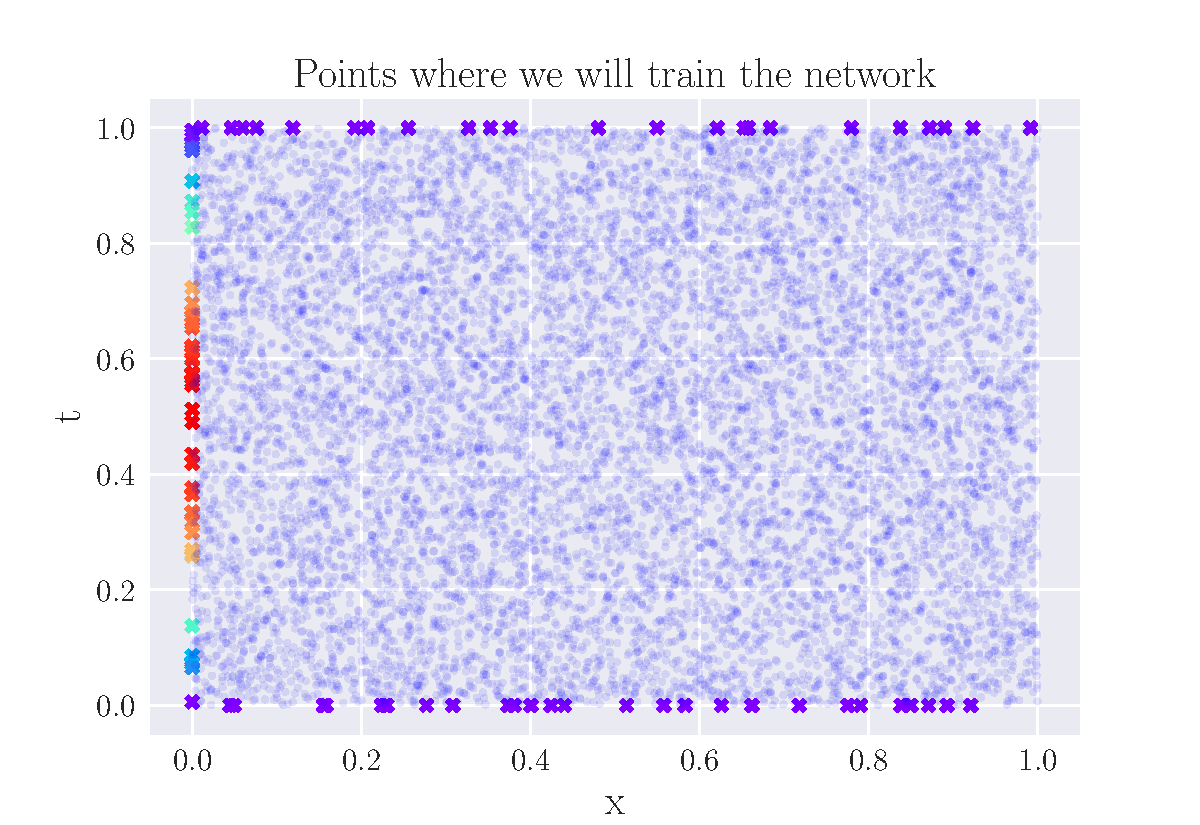
\includegraphics[width=\linewidth]{../output/plots/training_points.pdf}
	\caption{In this plot we highlight the data points used for training the neural network. Points on the boundary are highlighted, and we use $50$ points for $t=0$, and a total of $50$ points at $x=0$ and $x=1$, resulting in a total of $100$ boundary points. We use $10^4$ data points not at the boundary.} \label{fig:NN_training_points}
\end{figure}

\subsection{Forward Euler}

As discussed in the theory section, following equation \eqref{eq:stability}, $\alpha=0.5$ produce stable solutions for the diffusion equation. Throughout this report we will therefore use a time step of $\Delta t = \alpha \Delta x^2 = 0.5\cdot \Delta x^2$ for different choices of spatial resolution, and not consider other stability factors. We will limit our study to two spatial resolutions, namely $\Delta x = 0.1$ and $\Delta x = 0.01$.  

The first analysis we perform is the time evolution of the mean squared error (MSE) of the forward Euler solution. The MSE at a particular time step, $j$, is given as 
\begin{align} \label{eq:MSE}
	\mathrm{MSE_j} = \frac{1}{N}\sum_{i=0}^{N-1} (u_{p,i}^j - u_{a,i}^j)^2 
\end{align}
where $u_e$ denotes the analytical solution and $N$ is the number of spatial points. By construction the MSE should be zero at $t=0$. Subsequently, we expect an increasing MSE. Our boundary conditions results in the diffusion equation approaching $u(x,t)=0$ as $t$ increases, causing the MSE to eventually decline after a certain time. Combined with the unit test, this serves as a simple method of validating our result.  


\subsection{Comparing numerical results}
To proceed, we will study the results of the two numerical solvers at two different times, and we choose $t_1=0.1$ and $t_2=0.5$, where $u(x,t_1)$ is significantly curved and $u(x,t_2)$ is almost linear. These times will serve as the foundation for comparing the performance of our explicit numerical solver to that of the neural network. 

Using the aformentioned time points, we will compare the resulting MSE of the two methods, where we use both $\Delta x = 0.1$ and $\Delta x = 0.01$ for forward Euler. For the neural network we will only consider $\Delta x = 0.01$, but we will calculate the final MSE after four different traing iterations, namely $N_t\in\{500,\,1000,\,10^4,\,5\cdot10^4\}$, to see how increasing iterations affect the score.   

As a final study, we are going to plot the difference between the analytical solution and the two numerical solutions at $t_1$ and $t_2$, as a function of $x\in[0,\,1]$ 
\begin{align} \label{eq:absolute_difference}
	\Delta u(t) = u_{p}(t) - u_{a}(t),
\end{align}
where $u_p(t)$ is the numerical solution and $u_a(t)$ is the analytical solution. Our main purpose of this is to see whether the neural network can circumvent one of the major drawbacks of the forward Euler scheme, giving an output that is either consistently above or below the actual solution. For more volitale differential equations, such errors can propagate throughout the simulation, resulting in a poor fit. One potential advantage of using neural networks will thus be if it yields unbiased errors. 


\subsection{Finding eigenvalues}
The matrix we will consider for our initial analysis is a real symmetric matrix, $A$, with dimensions $(3\cross3)$ \footnote{We didn't realize that it should have been a $(6\cross6)$ matrix until after the report was finished. This has been cleared with Morten.}. In the end we will perform one simulation with a $(6\cross6)$ matrix to study differences for higher dimensions. 

Using the neural network model \eqref{eq:diff_eig} to find the eigenvalues of $A$ requires a trial solution \eqref{eq:NN_model} to initiate the network. The trial solution must fulfill the convergence property to guarantee that we end up with the eigenvalues, as mentioned in the theory section. Hence, we define the initial condition $x_0 \in \mathbb{R}^n$ to be a vector of randomly generated numbers between zero and one. Since we don't know the eigenspace corresponding to the largest eigenvalue a priori, we have no guarantee that the trial solution is non-orthogonal to the eigenspace corresponding to the largest eigenvalue. To increase the probability of non-orthogonality, we can add random perturbations.

Even though a non-zero trial solution is the only requirement for convergence, there are strategies for improving the \textit{rate} of convergence. If we have some preknowledge of a solution of the differential equation, incorporating this in the trial solution helps accelerate the learning of the neural network. The ODE \eqref{eq:diff_eig} is of first order with a term involving $dx/dt$ on one side and a term involving $x$ on the other. This is reminiscent of an exponential solution. Therefore, a smart initialization strategy of \eqref{eq:NN_model} is 

\begin{align}
	g_{\theta}(t) &= g_0(x(t)) + f[x(t),N(x, \theta)] \nonumber \\
	&= e^{-t}x_0 + (1 - e^{-t})N(x(t), \theta).
\end{align}

This expression fulfills the condition of a trial solution, namely that it must return the initial condition $x_0$ for time $t=0$. Once we have a trial solution we feed it to the neural network, which will calculate the gradient, $dx/dt$, and the resulting residual of $\eqref{eq:diff_eig}$. The MSE of the residual act as the loss function that is to be optimized through gradient descent. The accuracy of the final output of the neural network is assessed by comparing with the result of numpy's own eigenvalue solver. 

For comparison purposes, the forward euler scheme is initiated with the same initial condition $x_0$ as for the neural network model, and using the same temporal domain. Unless specified, a total time of $T=5$ is used, with a learning rate and number of epochs set to $0.005$ and $2000$ respectively, for the neural network.

For each simulation, we find the eigenvector, $\mathbf{v}_\mathrm{max}=(v_1,\,v_2,\,v_3)$, with the largest corresponding eigenvalue, $\lambda_\mathrm{max}$. We then plot the computed value of the three eigenvector components as a function of time, for both Forward Euler and Neural network. For a given simulation we also plot the time evolution of the Rayleigh quotient \eqref{eq:rayleigh_quotient}, for the two forementioned methods.   


\section{Results}

\subsection{Finding a suitable Neural network}

Table \ref{tab:NN_architecture_loss} shows the loss of the neural network after $500$ iterations for the three different network architectures. We see that $4$ hidden layers clearly yields the lowest value for the final loss. 
\begin{table}[h]
	\centering
	\begin{tabular}{|c|l|}
		\hline
		Architecture & Loss   \\ \hline
		$8\cross20$         & 0.0048 \\ \hline
		$4\cross20$         & 0.00079 \\ \hline
		$2\cross20$         & 0.0022 \\ \hline
	\end{tabular}
	\caption{Computed loss, equation \eqref{eq:NN_loss}, of the neural network after $500$ training iterations. The first number in the first column represents the number of hidden layers of the network, while the second number is the number of hidden nodes in each layer, which is $20$ for all three networks. $N_h=4$ yields the lowest MSE.}
	\label{tab:NN_architecture_loss}
\end{table}

The loss of the network as a function of iterations is shown in figure \ref{fig:Error_NN_architecture} for three different architectures, using $2$, $4$ and $8$ hidden layers for the upper left, upper right and lower left panel, respectively. 

\begin{figure}[h]
	\minipage{0.49\textwidth}
	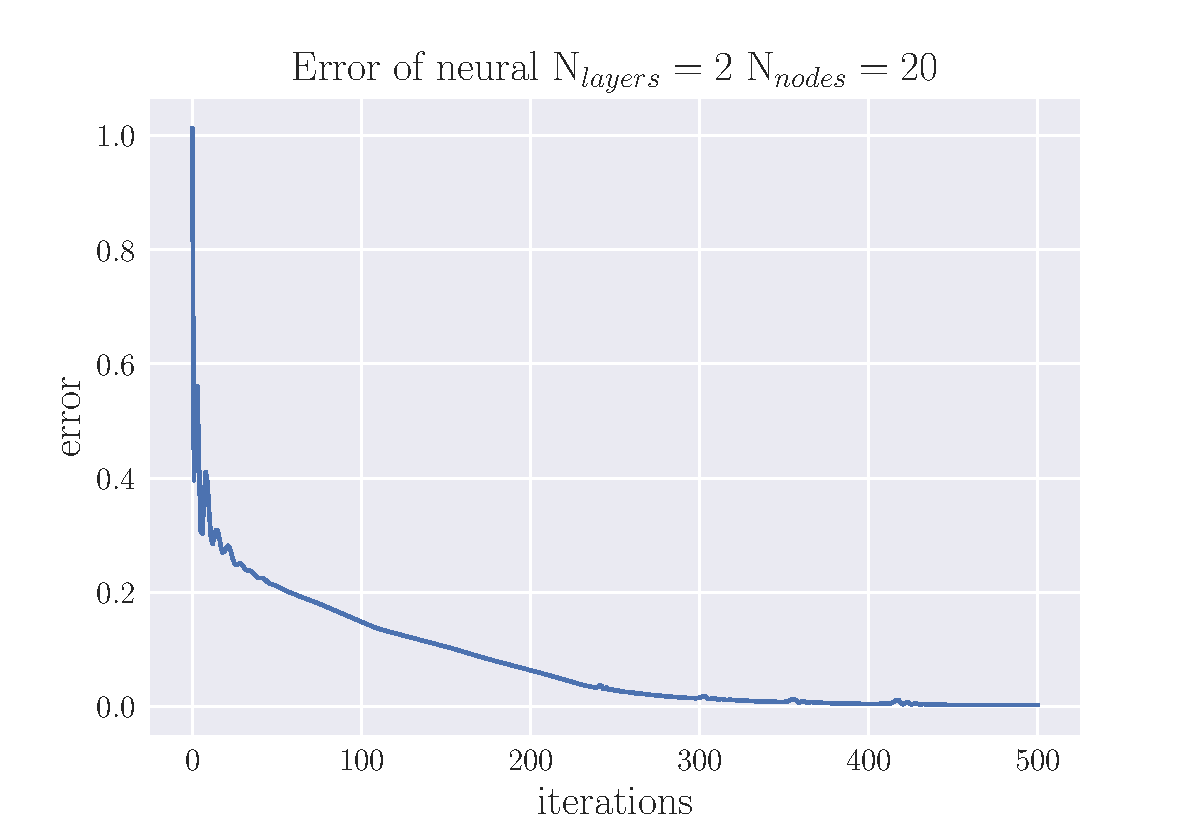
\includegraphics[width=\linewidth]{../output/plots/NN_diffusion_error_Nn20_Nh2.pdf}
	\endminipage\hfill
	\minipage{0.49\textwidth}
	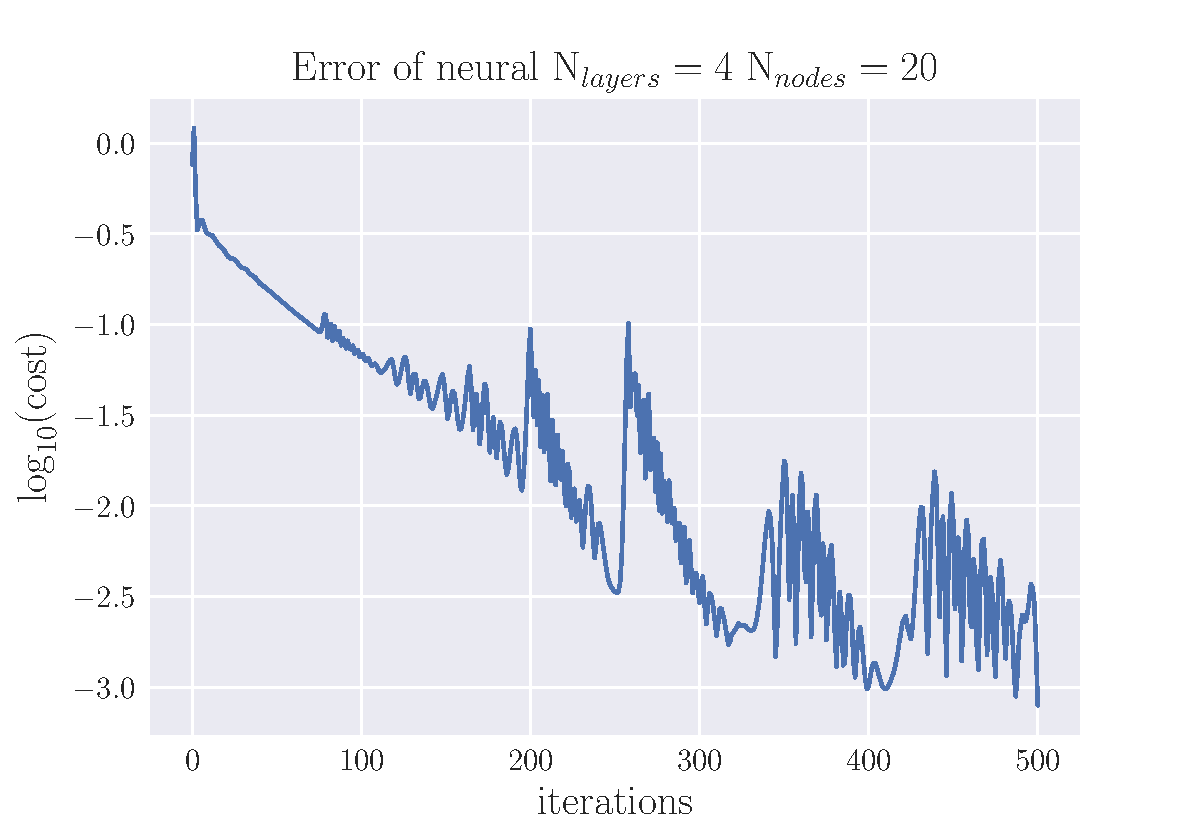
\includegraphics[width=\linewidth]{../output/plots/NN_diffusion_error_Nn20_Nh4.pdf}
	\endminipage\hfill
	\minipage{0.49\textwidth}
	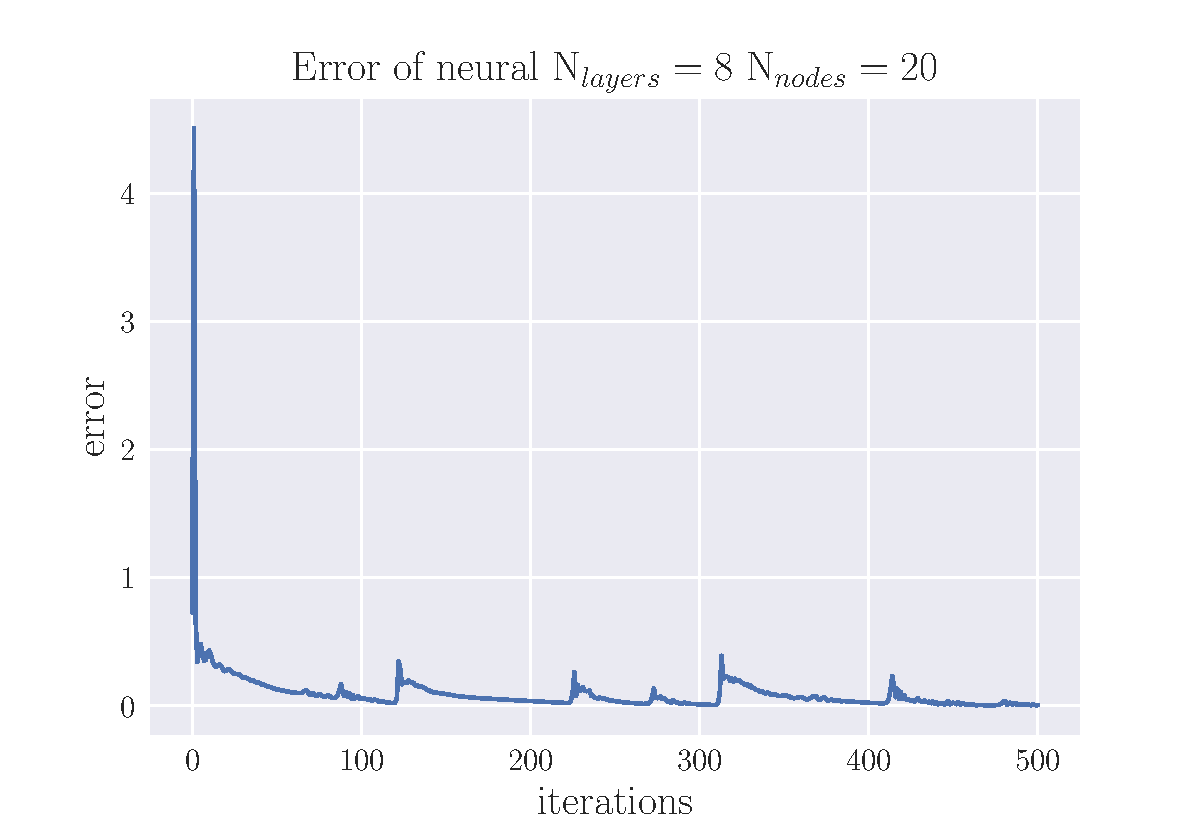
\includegraphics[width=\linewidth]{../output/plots/NN_diffusion_error_Nn20_Nh8.pdf}
	\endminipage\hfill
	\minipage{0.49\textwidth}
	\caption{Cost function of the neural network as a function of iterations, using $20$ hidden nodes in each network. The number of hidden layers in the network are $2,\,4$ and $8$, for the upper left, upper right and lower left panel, respectively.} \label{fig:Error_NN_architecture}
	\endminipage
\end{figure}

We notice large fluctuations of the loss for the network with $4$ hidden layers. Using logarithmic scales on the y-axes in figure \ref{fig:Error_NN_architecture}, the amplitudes of the oscillating losses appear bigger than they are in reality. As planned, we choose the network with $N_h=4$ for further analysis, as it yields the lowest MSE after $500$ iterations. A detailed study of different architectures is outside the scope of this report, and is nonetheless dependent of the particular PDE in question. 


Figure \ref{fig:NN_architecture_solution} shows the output of the neural network. We clearly see the exponential decay of the initial sine function, as expected, eventually flattening out, as $t\to1$.   
\begin{figure}[h]
	\centering
	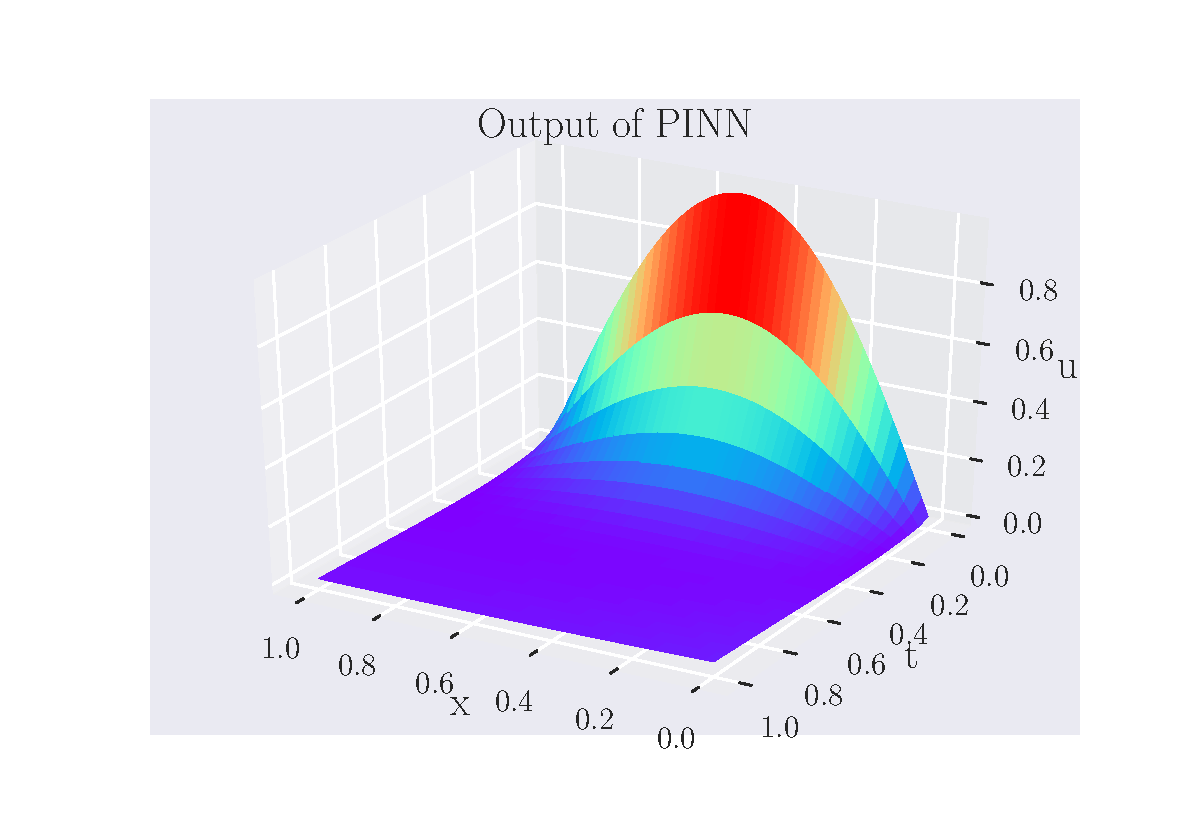
\includegraphics[width=\linewidth]{../output/plots/NN_diffusion_solution_Nn20_Nh4.pdf}
	\caption{The solution of the diffusion equation of the final neural network, with $N_h=4$ hidden layers.} \label{fig:NN_architecture_solution}
\end{figure}


\subsection{Error of Forward Euler scheme}

To assess the accuracy of our implemented numerical scheme, we need to test the how well the produced solution fits the analytical solution. Figure \ref{fig:FE_MSE} shows the MSE as function of time for the forward euler scheme (note the scaling of the y-axis). Keeping in mind that we choose the time step to give a stability factor of $\alpha=0.5$. 

The MSE in figure \ref{fig:FE_MSE} increases significantly for early time steps, reaching a peak at around $t_1=0.1$ and quickly reduces thereafter. At $t_2=0.5$ the MSE is significantly lower compared to $t_1$.  

\begin{figure}[h]
	\centering
	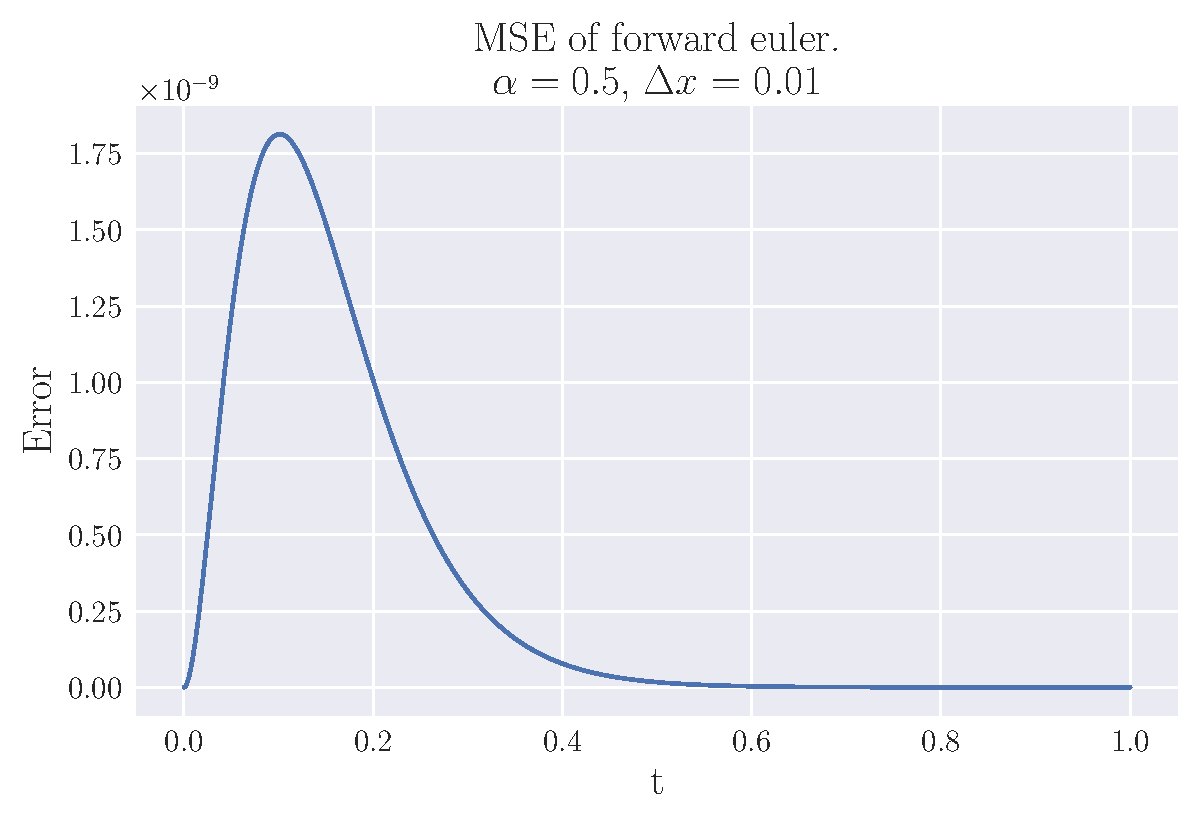
\includegraphics[scale=0.5]{../output/plots/MSE_FE_dx_001.pdf}
	\caption{Mean squared error of approximated solution by forward euler, using $\Delta x=0.01$ and time step $\Delta t$ dictated by the stability criterion \eqref{eq:stability}.}
	\label{fig:FE_MSE}
\end{figure}


\subsection{Comparison of error}
Table \ref{tab:NN_MSE_iterations} shows the resulting MSE of the neural network at $t_1$ and $t_2$ after four different number of training iterations. Except from an increase for $t_1$ when we go from $500$ to $1000$ training iterations, the MSE decreases as we increase the number of iterations. The increase is likely due to the fluctuations we saw in figure \ref{fig:Error_NN_architecture}. We will therefore use the output of the neural network after $5\cdot10^4$ training iterations for the remaining analysis on the diffusion equation, as this yielded the lowest MSE. 

\begin{table}[h]
	\centering
	\begin{tabular}{l|ll|}
		\cline{2-3}
		& \multicolumn{2}{l|}{Mean Square error} \\ \hline
		\multicolumn{1}{|l|}{Number of training iterations} & \multicolumn{1}{l|}{$t_1 = 0.1$} & $t_2 = 0.5$ \\ \hline
		\multicolumn{1}{|l|}{500}                           & \multicolumn{1}{l|}{0.0017}  & 0.0070  \\ \hline
		\multicolumn{1}{|l|}{1000}                          & \multicolumn{1}{l|}{0.015}   & 0.00055 \\ \hline
		\multicolumn{1}{|l|}{$10^4$}                          & \multicolumn{1}{l|}{$1.4\cdot 10^{-4}$}  & $9.5\cdot10^{-5}$  \\ \hline
		\multicolumn{1}{|l|}{$5\cdot10^4$}                        & \multicolumn{1}{l|}{$1.0\cdot10^{-6}$}        & $3.0\cdot10^{-6}$        \\ \hline
	\end{tabular}
	\caption{MSE of the neural network at two different times, using four different training iterations.}
	\label{tab:NN_MSE_iterations}
\end{table}



\begin{figure}[h]
	\centering
	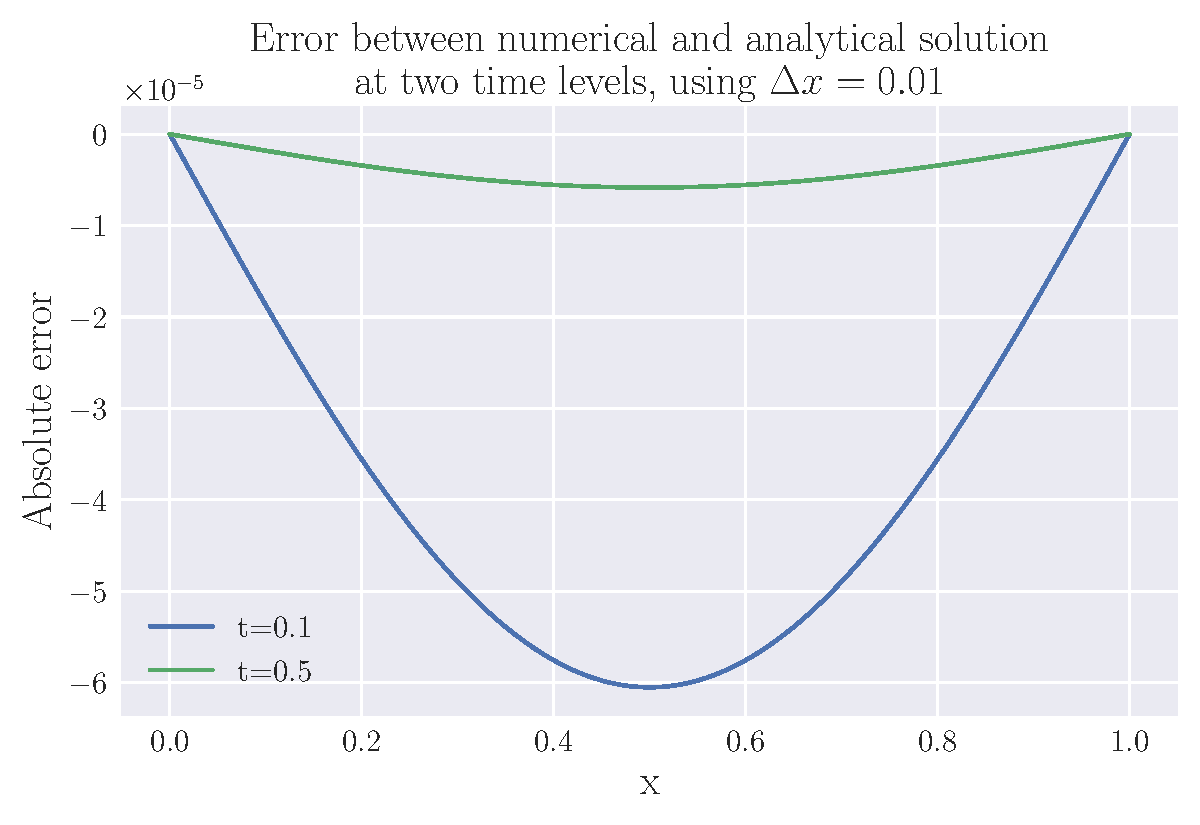
\includegraphics[width=0.75\linewidth]{../output/plots/error_FE_x_dx_001.pdf}
	\caption{The difference between the analytical solution of the diffusion equation and the solution obtained by forward euler at two different points in time.}
	\label{fig:FE_absolute_difference}
\end{figure}


\begin{figure}[h]
	\centering
	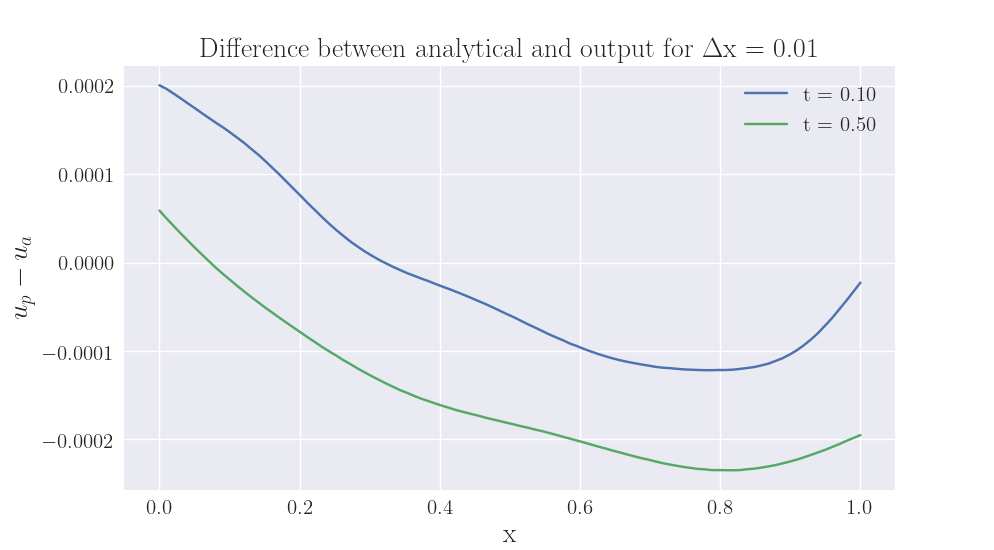
\includegraphics[width=0.8\linewidth]{../output/plots/final_compare_NN.png}
	\caption{The difference between the analytical solution of the diffusion equation and the solution obtained by the neural network at two different points in time, after $5\cdot10^4$ training iterations. The neural network has $N_h=4$ hidden layers.} \label{fig:NN_relative_error}
\end{figure}

Figure \ref{fig:FE_absolute_difference} shows the plot of equation \eqref{eq:absolute_difference}, i.e. the numerical solution of the diffusion equation from forward Euler, subtracted by the analytical solution in equation \eqref{eq:analytical_solution_diffusion}. The corresponding plot for the neural network is shown in figure \ref{fig:NN_relative_error}. Using $\Delta x=0.1$ for forward Euler yielded an identically shaped plot as figure \ref{fig:FE_absolute_difference}, but with increased values on the $y$-axis, and we have therefore chosen to omit it. 

In figure \ref{fig:FE_absolute_difference} we see the expected feature of forward euler, lying below the analytical solutions throughout the simulation. Comparing with figure \ref{fig:NN_relative_error}, we note that at $t_1=0.1$ the difference is positive for $x\lesssim0.3$, while it is negative for larger $x$ values. Similarly, we get a positive difference at $t_2=0.5$ for the lower values of $x$. Although there is a slight bias in the difference from the neural network, neither time points yielded a completely negative solution.   

Table \ref{tab:MSE_compare} compares the MSE obtained for forward euler and neural network at two selected time steps $t$. With forward Euler we have included both spatial steps $\Delta x$, while we only consider $\Delta x=0.01$ for the neural network. 

\begin{table}[h]
	\centering
	\begin{tabular}{l|cc|cc|}
		\cline{2-5}
		& \multicolumn{2}{c|}{\textbf{$\Delta x=0.1$}}           & \multicolumn{2}{c|}{\textbf{$\Delta x=0.01$}}           \\ \cline{2-5} 
		& \multicolumn{1}{l|}{\textbf{FE}}         & \textbf{NN} & \multicolumn{1}{l|}{\textbf{FE}}          & \textbf{NN} \\ \hline
		\multicolumn{1}{|l|}{\textbf{$t_1=0.1$}} & \multicolumn{1}{l|}{$1.72\cdot 10^{-5}$} & -            & \multicolumn{1}{l|}{$1.81\cdot 10^{-9}$}  & $1.0\cdot10^{-6}$            \\ \hline
		\multicolumn{1}{|l|}{\textbf{$t_2=0.5$}} & \multicolumn{1}{l|}{$1.50\cdot 10^{-7}$} & -            & \multicolumn{1}{l|}{$1.69\cdot 10^{-11}$} & $3.0\cdot10^{-6}$             \\ \hline
	\end{tabular}
\caption{MSE as function of spatial step $\Delta x$ for two different time levels, for forward euler scheme and neural network. Forward euler is abbreviated as FE and neural network as NN.}
\label{tab:MSE_compare}
\end{table}

In table \ref{tab:MSE_compare} we see that forward Euler yields much lower MSE values for $\Delta x = 0.01$ than the neural network. For $t_1=0.1$ and $t_2=0.5$ the MSE of the neural network exceeds the MSE of forward Euler by factors of $\sim10^3$ and $\sim10^5$, respectively. At $t_2=0.5$ the MSE of the neural network with $\Delta x = 0.01$ is approximately $20$ times greater than the MSE of forward Euler with $\Delta x=0.1$, i.e. $10$ times fewer data points. 

\subsection{Eigenvalue problem}


\begin{figure}[h]
	\centering
	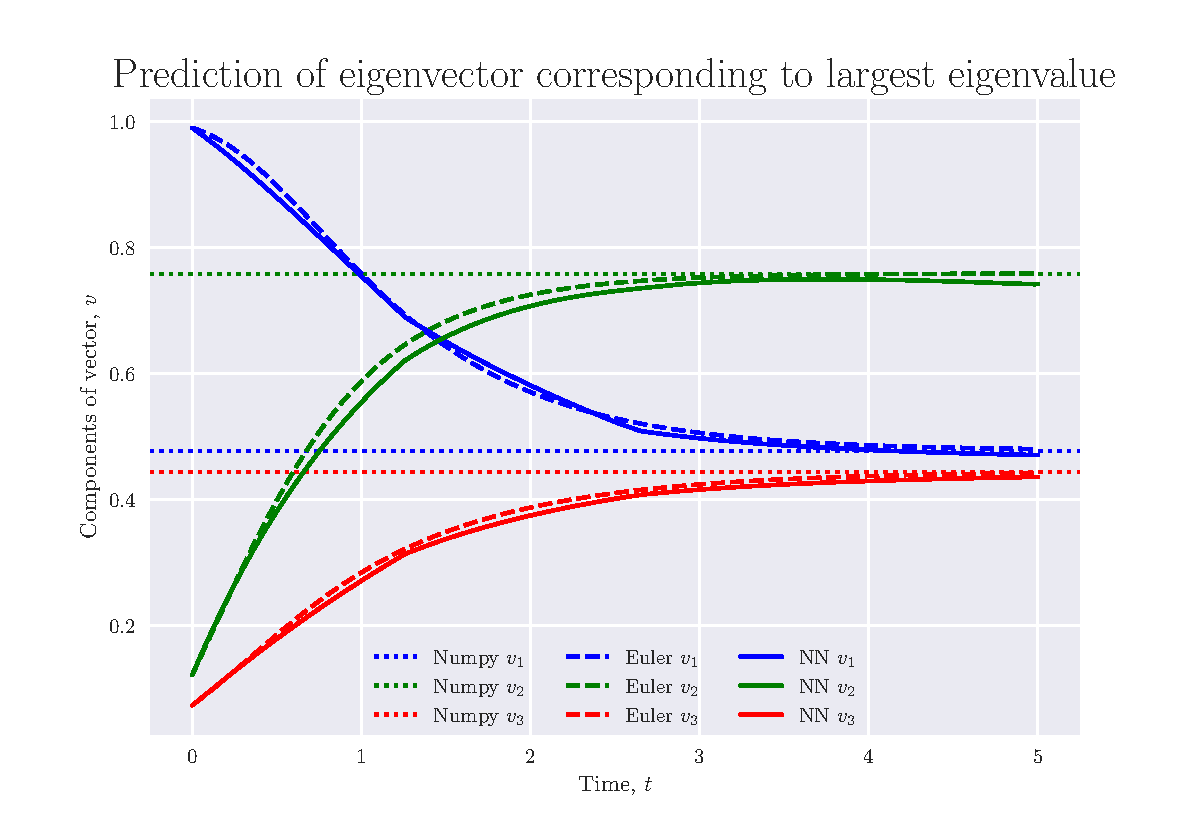
\includegraphics[scale=0.75]{../output/plots/eigvec_T5_N1000.pdf}
	\caption{Predictions by forward euler (FE) and neural network (NN) of the eigenvector corresponding to the largest eigenvalue of a real, symmetric $3\times 3$ matrix. The horizontal dotted lines are the components of the eigenvector as found by NumPy.}
	\label{fig:eigvec_T5_N1000}
\end{figure}

\begin{figure}[h]
	\centering
	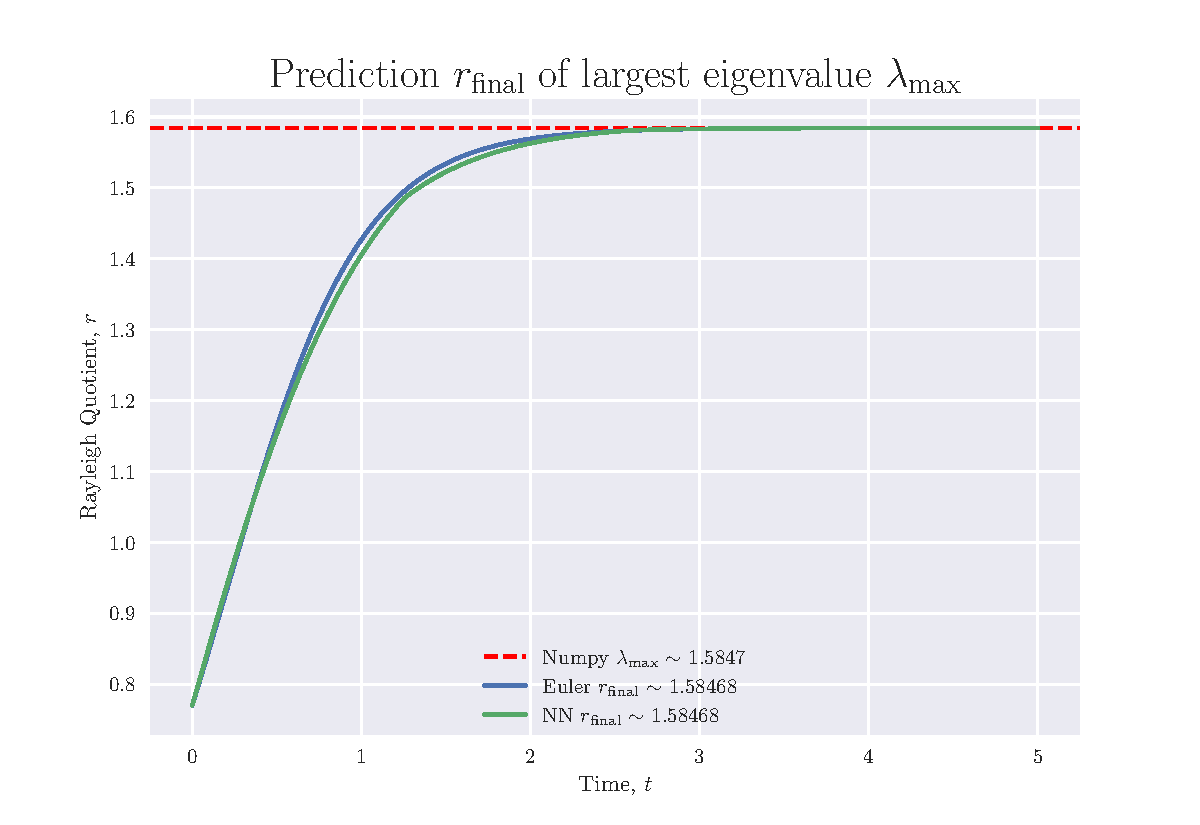
\includegraphics[scale=0.75]{../output/plots/eigval_T5_N1000.pdf}
	\caption{Rayleigh quotients of forward euler (FE) and neural network (NN) representing predictions of the largest eigenvalue of a real, symmetric $3\times 3$ matrix. The horizontal dotted line is the largest eigenvalue as found by NumPy.}
	\label{fig:eigval_T5_N1000}
\end{figure}

Figure \ref{fig:eigvec_T5_N1000} shows predictions of the eigenvector corresponding to the largest eigenvalue of a symmetric $(3\times 3)$ matrix $A$ of randomly assigned values between zero and one. The simulation is run for a total time of $T=5$ with $N=1000$ estimations in time, providing a time step of $\Delta t = 0.005$. The prediction from both forward euler and neural network converges to the true eigenvector, as obtained from NumPy. The largest eigenvalue is shown in Figure \ref{fig:eigval_T5_N1000} together with the rayleigh quotients estimated by forward euler and the neural network.

Note that some of the figures that follow are horizontally aligned for readability purposes. This means that the axes labels are small, but we inform that the labels are identical to those of figure \ref{fig:eigvec_T5_N1000} and figure \ref{fig:eigval_T5_N1000}. The plots are only meant to illustrate trends as we alter simulation parameters. 

\begin{figure}[h]
	
	\centering
	\begin{subfigure}{0.49\textwidth}
		\centering
		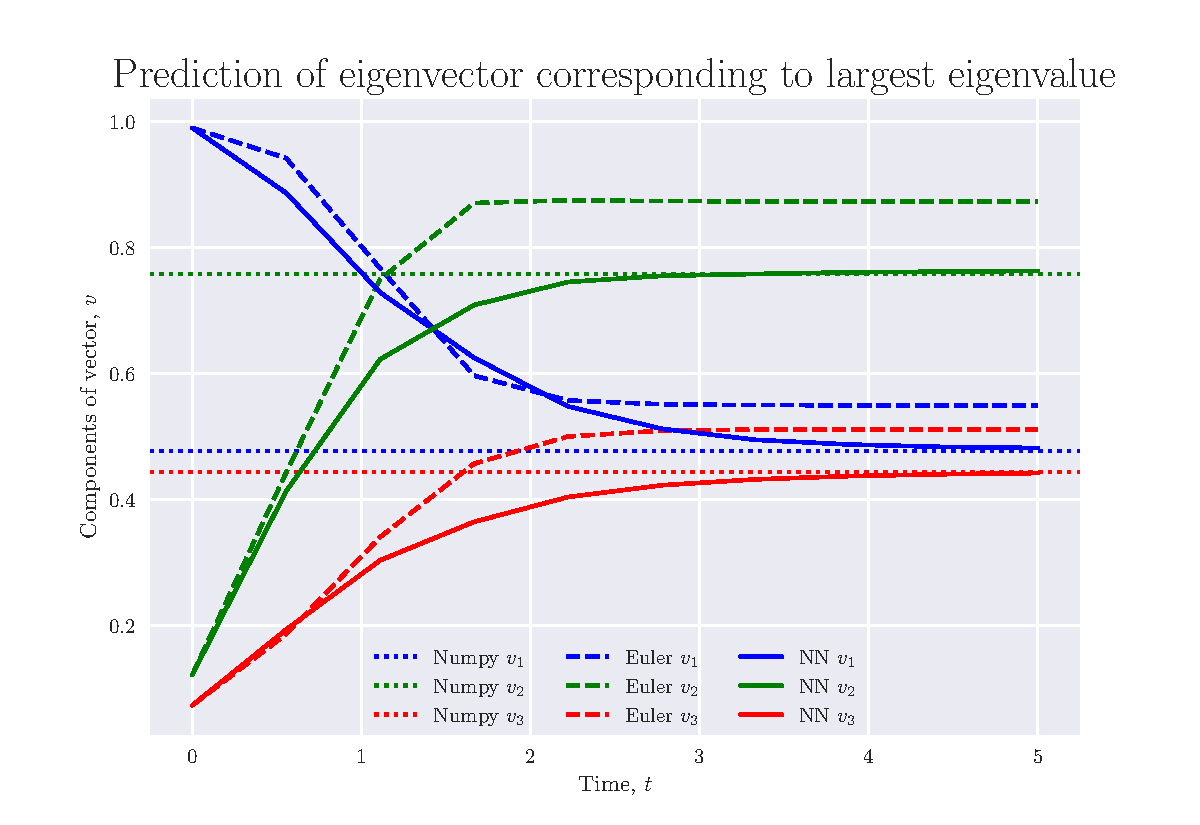
\includegraphics[width=\textwidth]{../output/plots/eigvec_T5_N10.pdf}
		\caption{Eigenvectors}
		\label{fig:eigvec_T5_N10}
	\end{subfigure}
	\hfill
	\begin{subfigure}{0.49\textwidth}
		\centering
		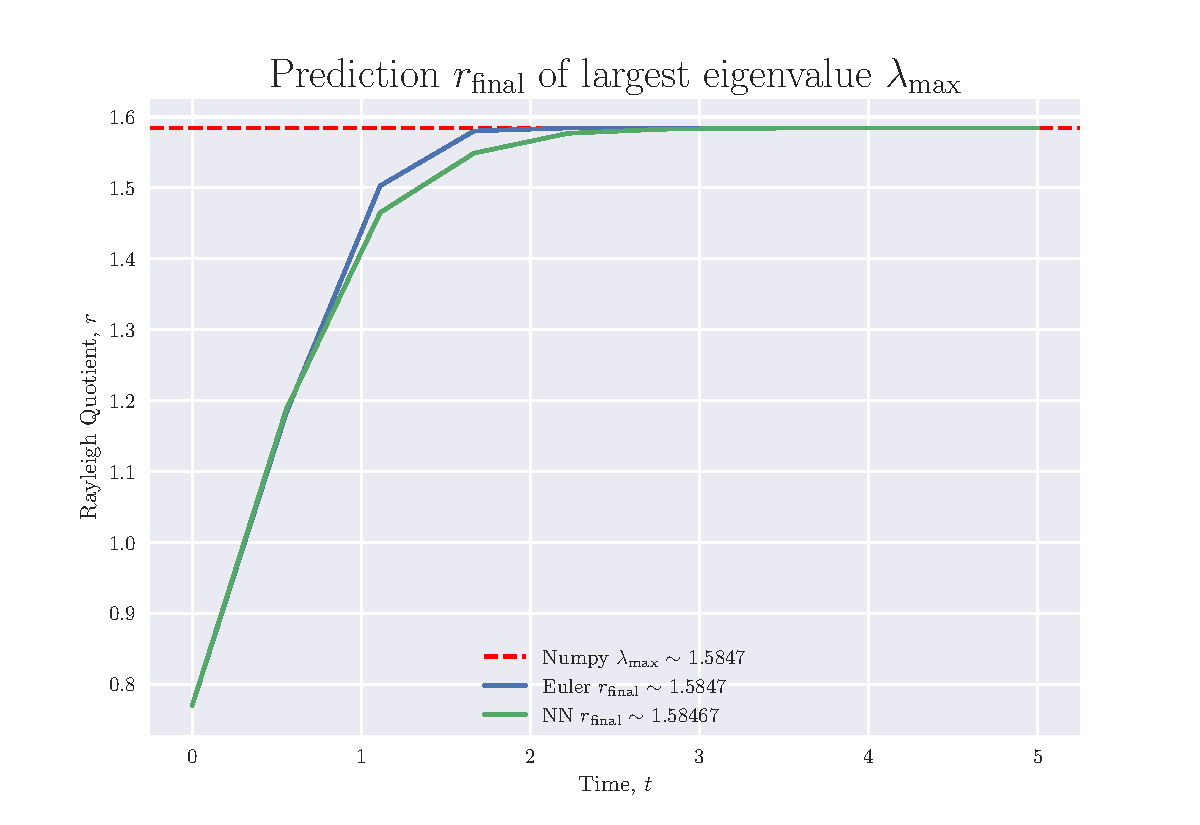
\includegraphics[width=\textwidth]{../output/plots/eigval_T5_N10.pdf}
		\caption{Rayleigh quotients}
		\label{fig:eigval_T5_N10}
	\end{subfigure}
	\caption{Predictions by forward euler (FE) and neural network (NN) of largest eigenvalue and corresponding eigenvector of a real, symmetric $3\times 3$ matrix, using a time step $\Delta t = 0.5$. The $x$ and $y$ axes are identical to those in figure \ref{fig:eigvec_T5_N1000} and \ref{fig:eigval_T5_N1000}}
	\label{fig:eig_T5_N10}
\end{figure}



Figure \ref{fig:eigvec_T5_N10} shows predictions of the same eigenvector of the same matrix $A$ in Figure \ref{fig:eigvec_T5_N1000} but with a time step of $\Delta t = 0.5$. The largest eigenvalue and rayleigh quotients are shown in Figure \ref{fig:eigval_T5_N10}.
The graphs are less smooth due to a larger timestep and fewer estimates. 

\begin{figure}[h]
	\centering
	\begin{subfigure}{0.49\textwidth}
		\centering
		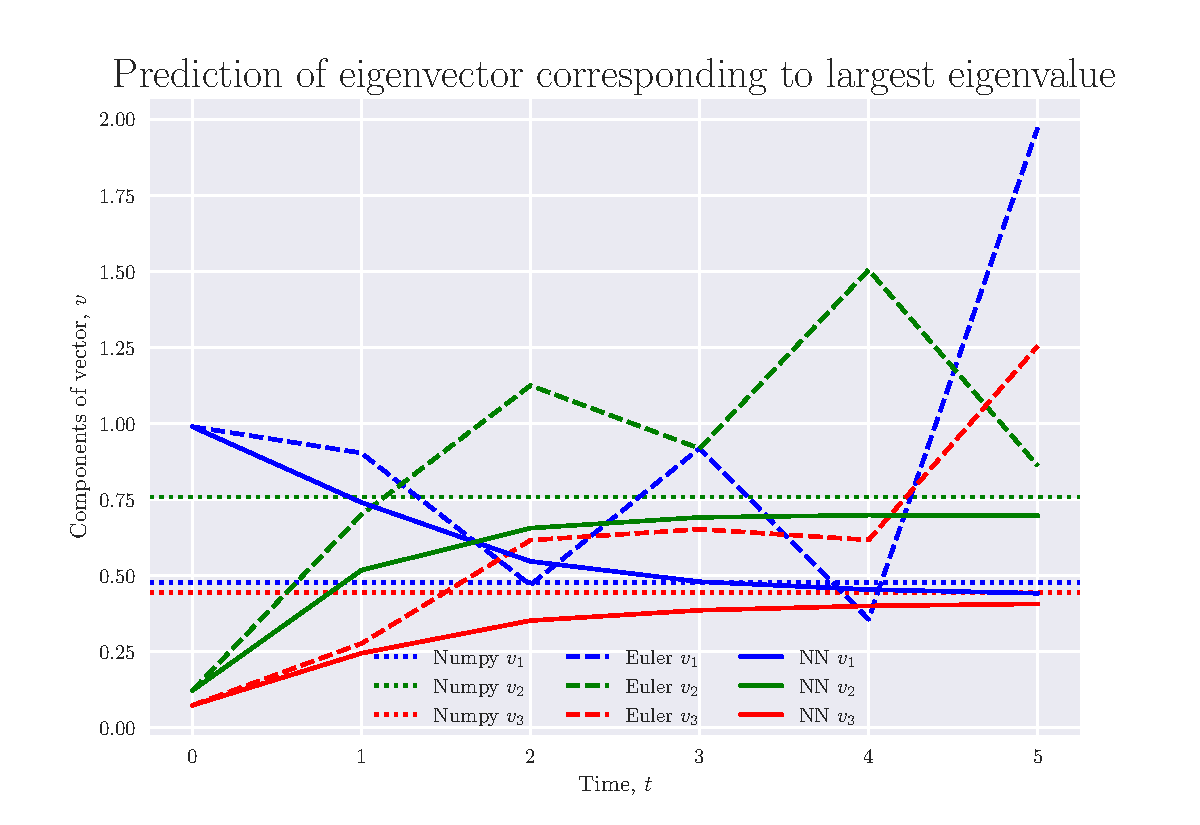
\includegraphics[width=\textwidth]{../output/plots/eigvec_T5_N6.pdf}
		\caption{Eigenvectors}
		\label{fig:eigvec_T5_N6}
	\end{subfigure}
	\hfill
	\begin{subfigure}{0.49\textwidth}
		\centering
		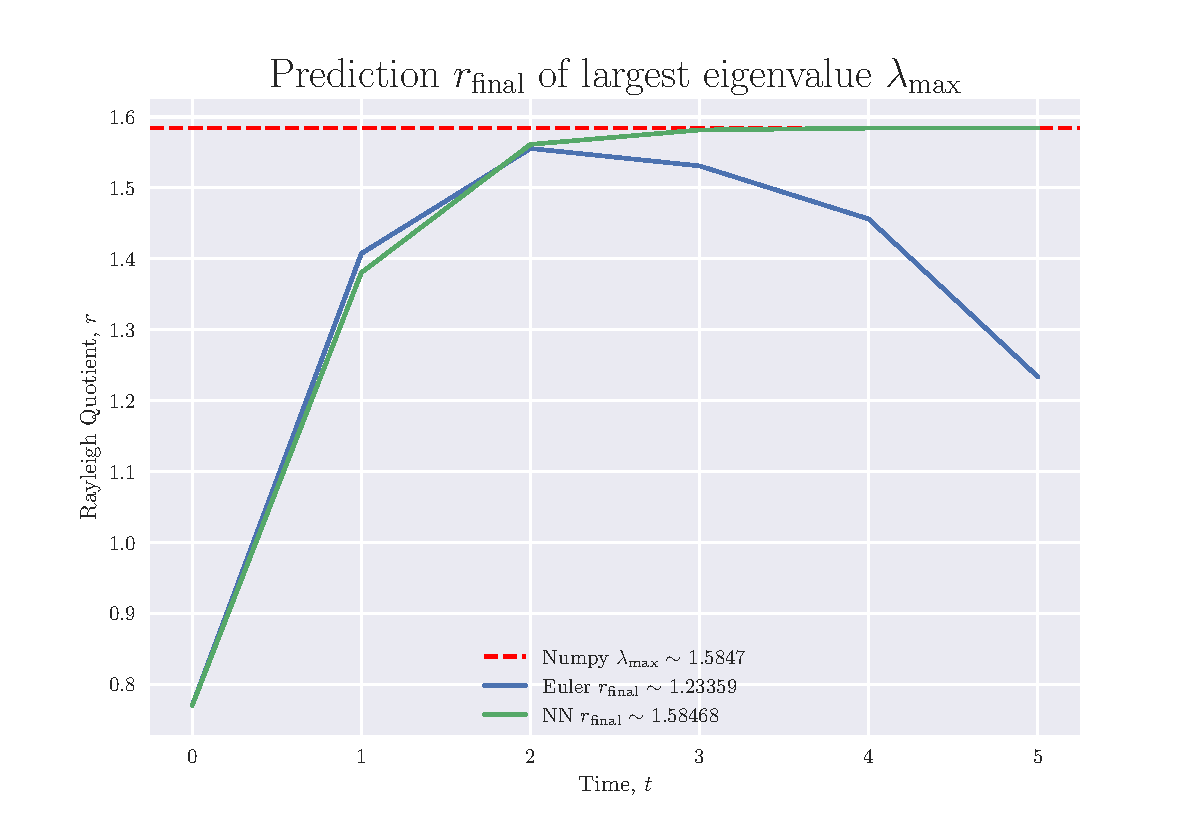
\includegraphics[width=\textwidth]{../output/plots/eigval_T5_N6.pdf}
		\caption{Rayleigh quotients}
		\label{fig:eigval_T5_N6}
	\end{subfigure}
	\caption{Predictions of largest eigenvalue and corresponding eigenvector by forward euler and neural network for a real, symmetric $3\times 3$ matrix. A time step of $\Delta t = 0.83$ is used. Other than increased eigenvector component values for forward Euler on the left panel, the $x$ and $y$ axes are identical to those in figure \ref{fig:eigvec_T5_N1000} and \ref{fig:eigval_T5_N1000}}
	\label{fig:eig_T5_N6}
\end{figure}

Results of a further increase in the time step is shown in Figure \ref{fig:eig_T5_N6}, using $\Delta t= 0.83$ corresponding to $N=6$ estimations, where the left panel shows the eigenvector components and the right panel shows the associated Rayleigh quotients. Note that diverging eigenvector components in figure \ref{fig:eigvec_T5_N6} have altered the y-axis, but is otherwise similar to that of previous figures. 

\begin{figure}[h]
	
	\centering
	\begin{subfigure}{0.49\textwidth}
		\centering
		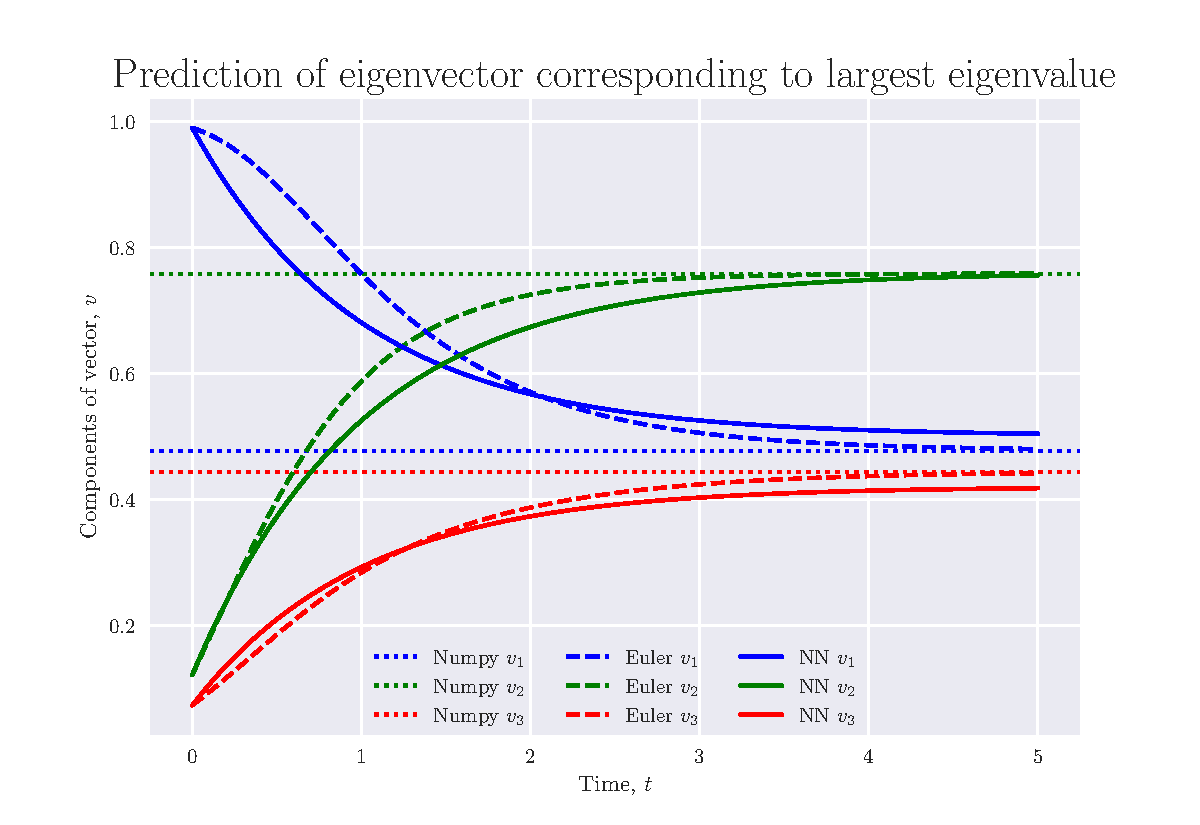
\includegraphics[width=\textwidth]{../output/plots/eigvec_T5_N1000_eta01.pdf}
		\caption{Eigenvectors}
		\label{fig:eigvec_T5_N1000_eta01}
	\end{subfigure}
	\hfill
	\begin{subfigure}{0.49\textwidth}
		\centering
		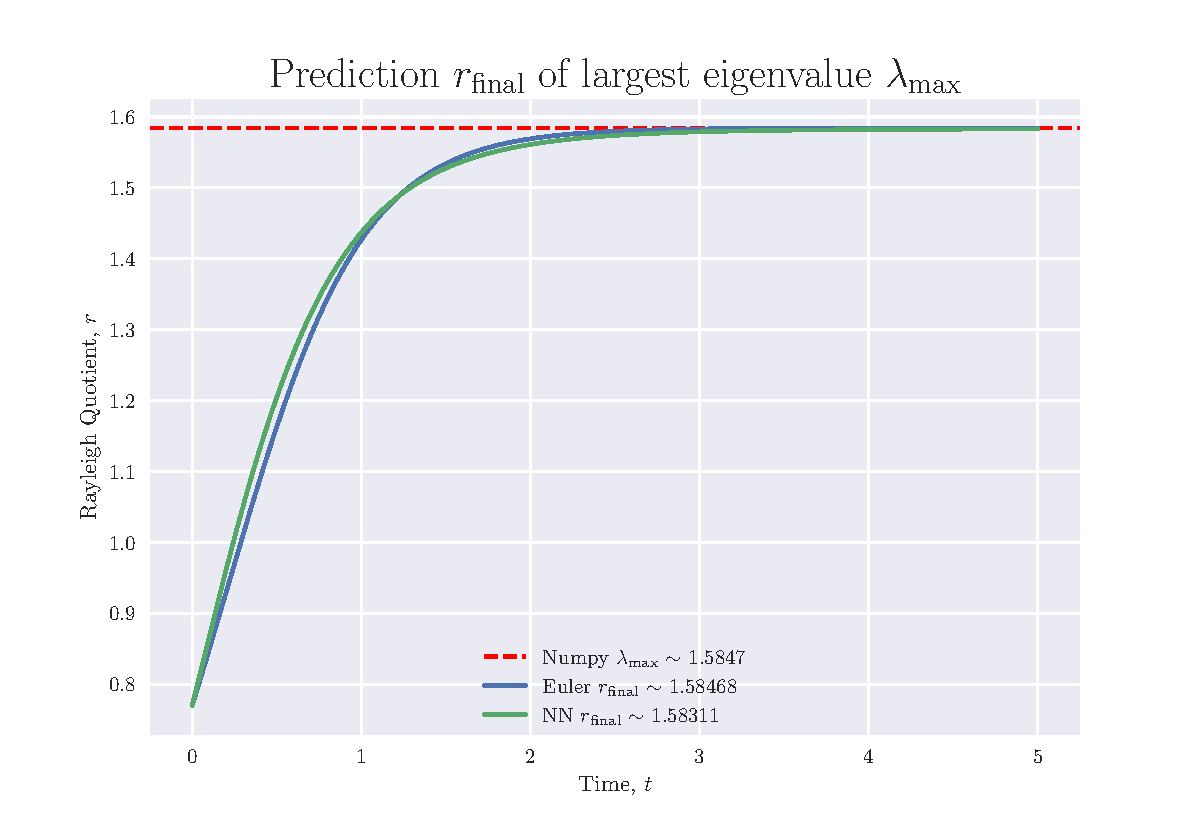
\includegraphics[width=\textwidth]{../output/plots/eigval_T5_N1000_eta01.pdf}
		\caption{Rayleigh quotients}
		\label{fig:eigval_T5_N1000_eta01}
	\end{subfigure}
	\caption{Predictions of largest eigenvalue and corresponding eigenvector by forward euler and neural network for a real, symmetric $3\times 3$ matrix, using a learning rate of $0.1$ and a time step $\Delta t = 0.005$. The $x$ and $y$ axes are identical to those in figure \ref{fig:eigvec_T5_N1000} and \ref{fig:eigval_T5_N1000}}
	\label{fig:eig_T5_N1000_eta01}
\end{figure}

\begin{figure}[h]
	
	\centering
	\begin{subfigure}{0.49\textwidth}
		\centering
		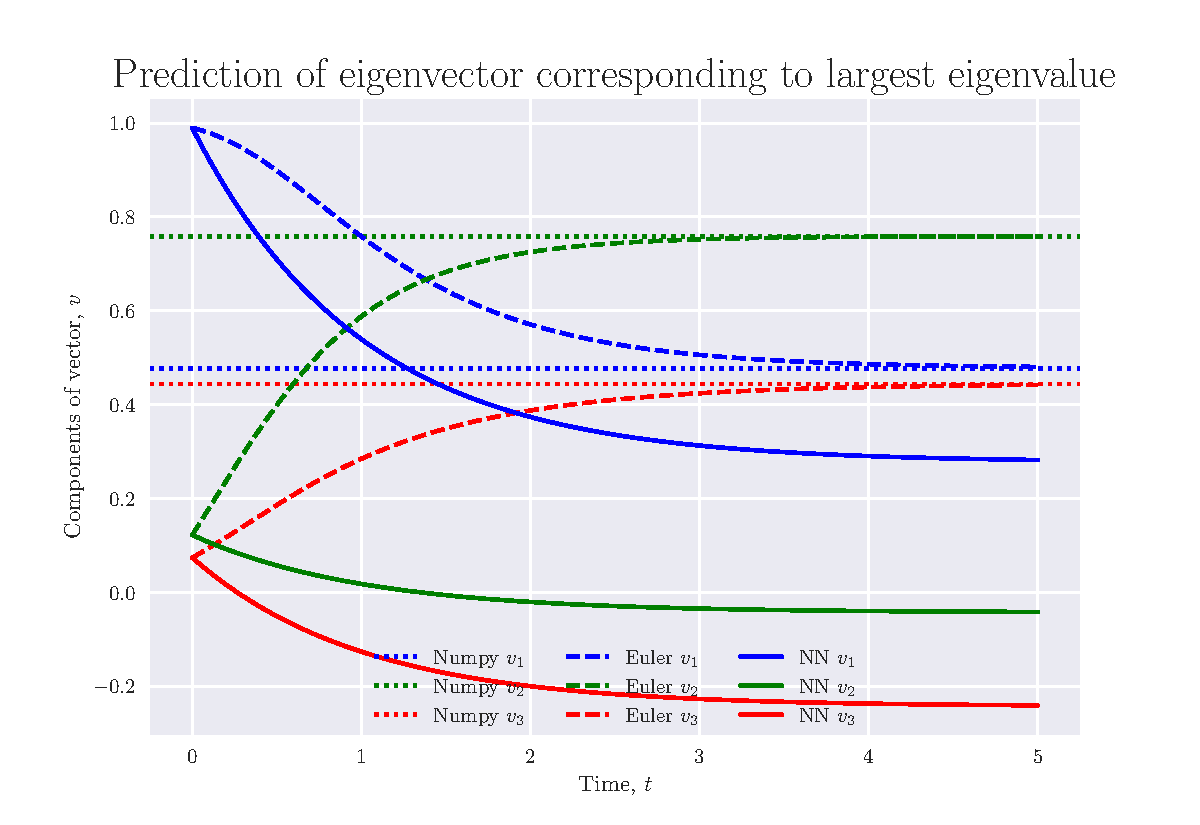
\includegraphics[width=\textwidth]{../output/plots/eigvec_T5_N1000_epochs50.pdf}
		\caption{Eigenvectors}
		\label{fig:eigvec_T5_N1000_epochs50}
	\end{subfigure}
	\hfill
	\begin{subfigure}{0.49\textwidth}
		\centering
		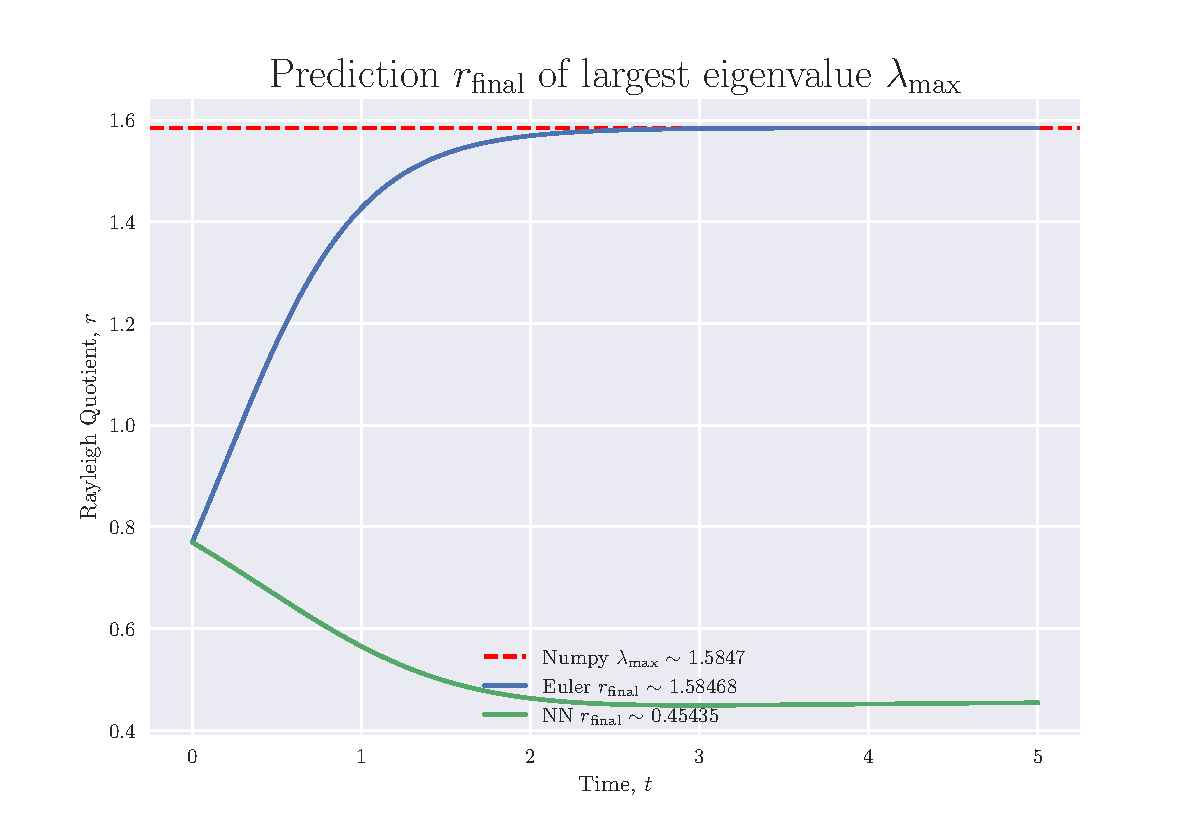
\includegraphics[width=\textwidth]{../output/plots/eigval_T5_N1000_epochs50.pdf}
		\caption{Rayleigh quotients}
		\label{fig:eigval_T5_N1000_epochs50}
	\end{subfigure}
	\caption{Predictions of largest eigenvalue and corresponding eigenvector by forward euler and neural network for a real, symmetric $3\times 3$ matrix, using a learning rate of $0.1$, $50$ epochs and a time step $\Delta t = 0.005$. Other than negative eigenvector components in the left panel, and lower Rayleigh quotient in the right panel, the $x$ and $y$ axes are identical to those in figure \ref{fig:eigvec_T5_N1000} and \ref{fig:eigval_T5_N1000}}
	\label{fig:eig_T5_N1000_epochs50}
\end{figure}


Adjusting hyperparameters of the neural network has also been investigated. Figure \ref{fig:eigvec_T5_N1000_eta01} shows the predicted eigenvector using a time step of $\Delta t = 0.005$ and a learning rate of $0.1$. The associated rayleigh quotients is shown in Figure \ref{fig:eigval_T5_N1000_eta01}. Predictions of the same eigenvector is shown in Figure \ref{fig:eigvec_T5_N1000_epochs50}, with the learning rate retained at $0.1$ but the number of epochs reduced from $2000$ to $50$. The associated rayleigh quotients are shown in Figure \ref{fig:eigval_T5_N1000_epochs50}.

\begin{figure}[h]
	\centering
	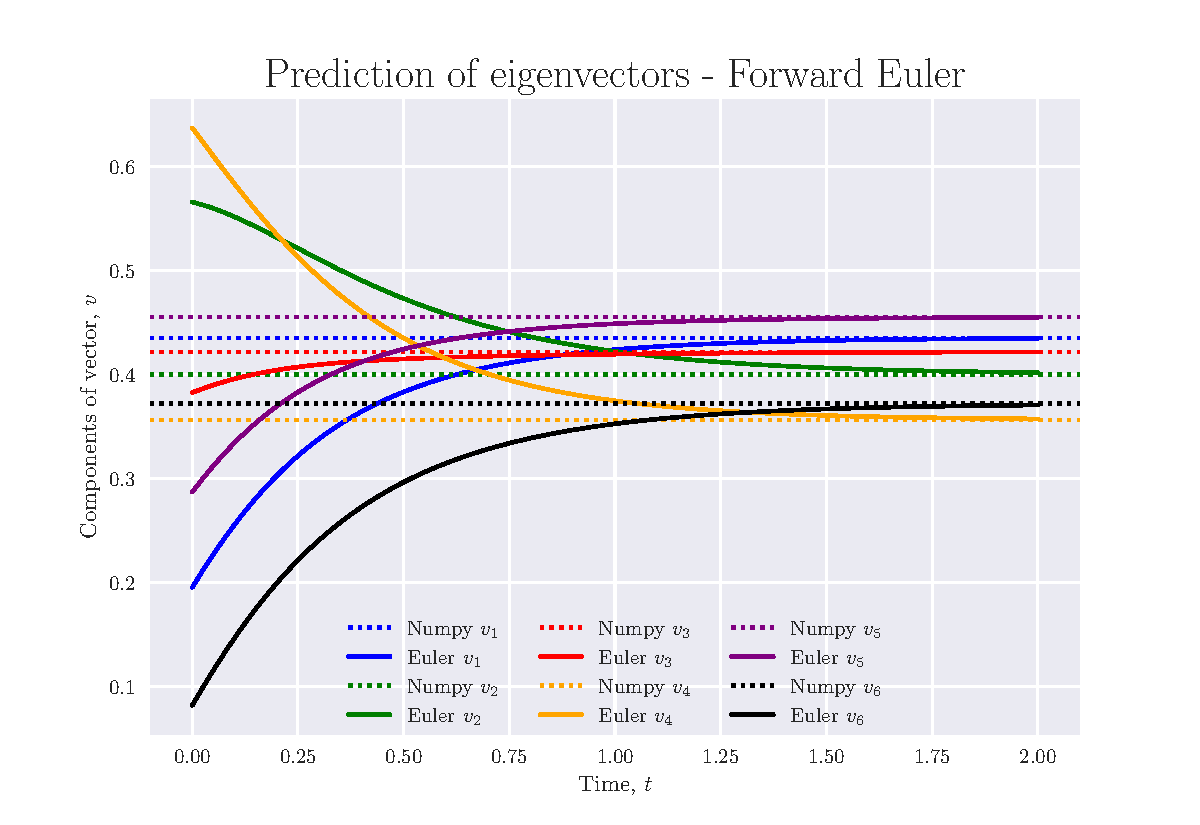
\includegraphics[scale=0.6]{../output/plots/FE_eigvec_T2_N1000_dim6.pdf}
	\caption{Predictions of eigenvector corresponding to the largest eigenvalue for a real, symmetric $6\times 6$ matrix using Forward Euler. A time step of $\Delta t = 0.005$ and a total time $T=2$ is used.}
	\label{fig:FE_eigvec_T2_N1000_dim6}
\end{figure}

\begin{figure}[h]
	\centering
	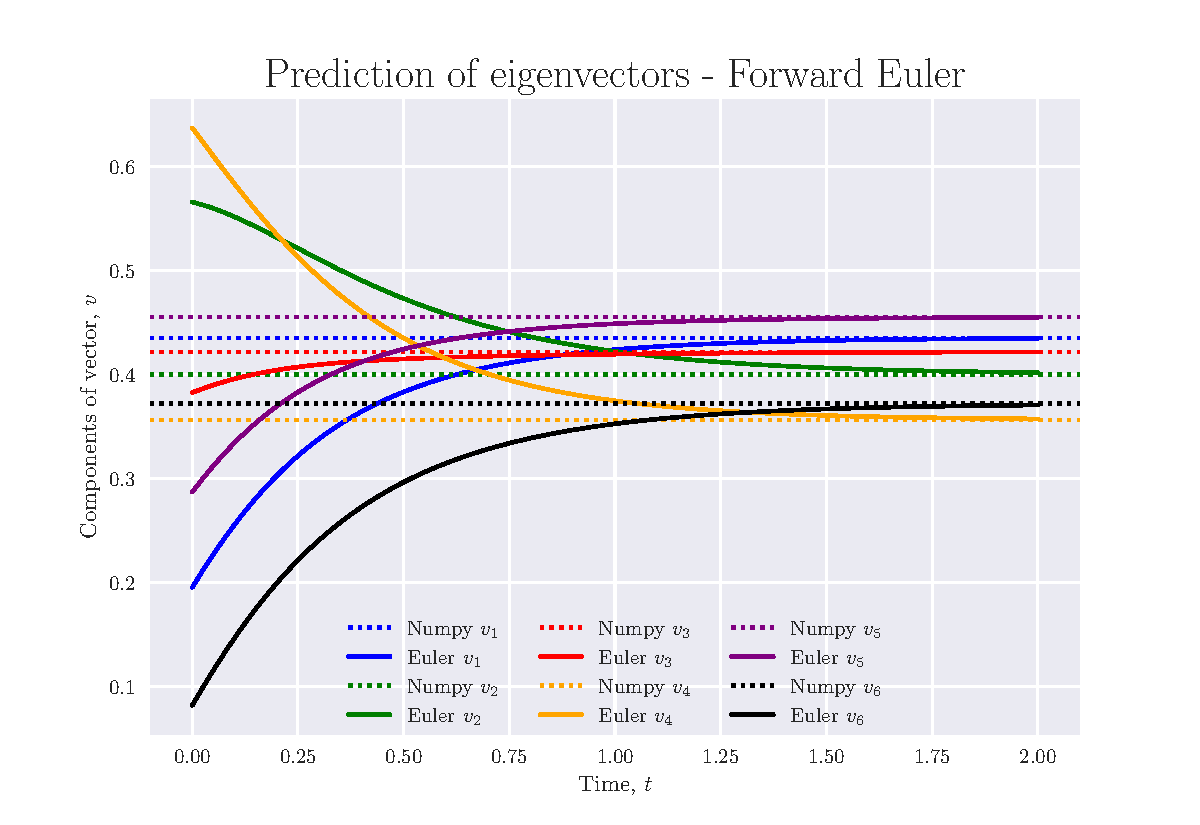
\includegraphics[scale=0.6]{../output/plots/NN_eigvec_T2_N1000_dim6.pdf}
	\caption{Predictions of eigenvector corresponding to the largest eigenvalue for a real, symmetric $6\times 6$ matrix using Neural network. A time step of $\Delta t = 0.005$ and a total time $T=2$ is used.}
	\label{fig:NN_eigvec_T2_N1000_dim6}
\end{figure}

\begin{figure}[h]
	\centering
	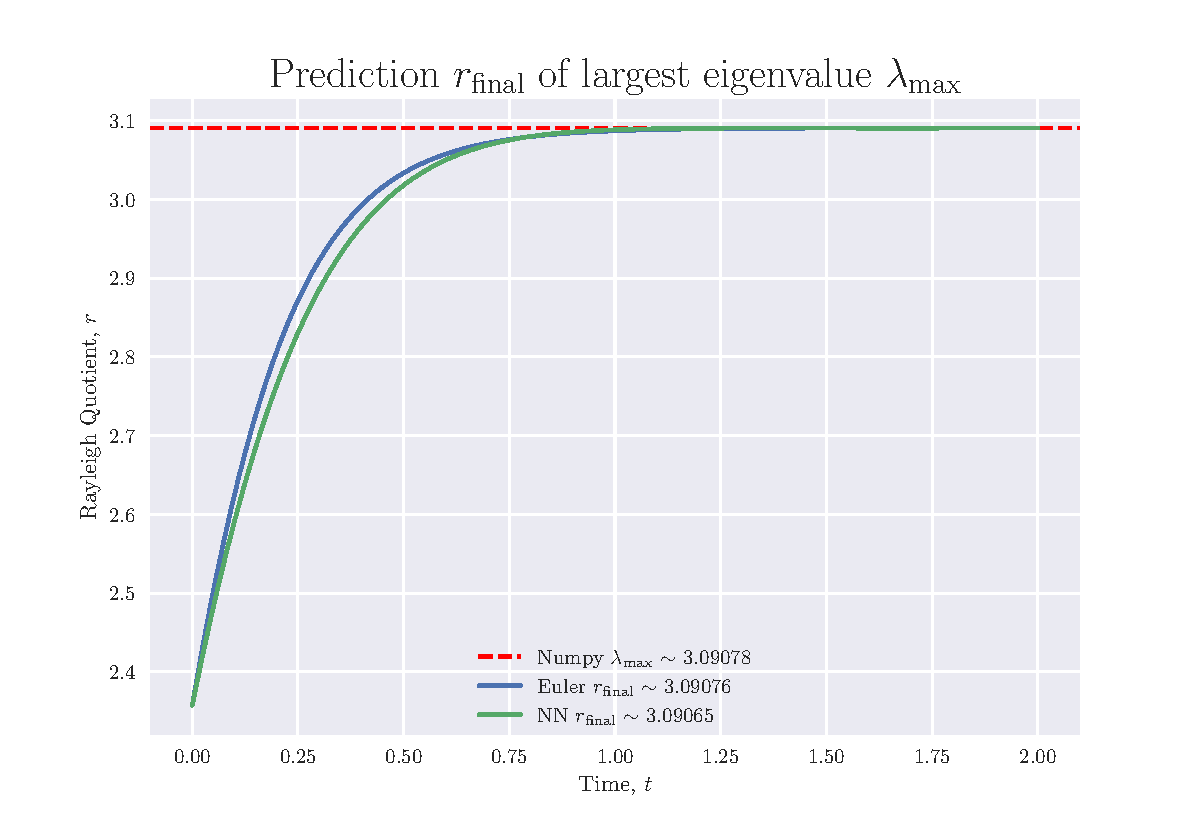
\includegraphics[scale=0.6]{../output/plots/eigval_T2_N1000_dim6.pdf}
	\caption{Rayleigh quotient corresponding to the largest eigenvalue of a real, symmetric $6\times 6$ matrix.}
	\label{fig:eigval_T2_N1000_dim6}
\end{figure}

An additional simulation using a $6\times 6$ matrix has also been conducted. Figure \ref{fig:FE_eigvec_T2_N1000_dim6} and Figure \ref{fig:NN_eigvec_T2_N1000_dim6} shows the predicted eigenvector for forward euler and neural network, repsectively, and Figure \ref{fig:eigval_T2_N1000_dim6} the rayleigh coefficient corresponding to the largest eigenvalue of a $6\times 6$ symmetric matrix. A time step of $\Delta t = 0.005$ have been used and a total time of $T=2$. The reason for the latter choice is based on experiments with a $(6 \cross 6)$ matrix indicating convergence long before $T=5$. Simulating for a shorter time period better illustrates the convergence of the eigenvector.

The reason for the latter choice is based on the previous simulations with $\Delta t=0.005$, as both forward euler and neural network converge long before $T=5$. Reducing the simulation time makes it easier to illustrate the convergence property of the six eigenvector components.
 
\clearpage
\section{Discussion}

\subsection{Solving the diffusion equation with Forward Euler}

We don't have much to discuss when it comes to implementation of forward Euler. All results was as expected, namely decreasing the time step $\Delta t$ gave us a lower MSE, to get it even lower one could experiment with lower values of $\Delta t$. Also, as we discussed, the output was constantly below the analytical solution for both timesteps in figure \ref{fig:FE_absolute_difference}.

\subsection{Solving the diffusion equation with a neural network}

When solving the diffusion equation with the neural network we only explored how the number of hidden layers affected the loss function. There are several things one could study to optimize the results. For instance different activation function, number of hidden nodes in each layer, learning rate and initialization of weights and biases. Also since the initial and boundary conditions are known, it would be favorable to find a way to implement this, so that the network returns correct values at those points. This was only implemented in the loss function as regularization terms. 

One thing we noticed was that the loss in figure \ref{fig:Error_NN_architecture}, fluctuates instead of decreasing monotonically. We believe this could due to the use of Adam optimizer, as discussed by Kingma et. al. \cite{kingma2017adam}. The reason for this is due to the stochastic nature of Adam.

\subsection{Comparison between Forward Euler and neural network}

One noteworthy aspect of the neural network results, was that the MSE at $t_1=0.1$ was three times lower than it was at $t_2=0.5$. This is easily seen from figure \ref{fig:NN_relative_error}, where the difference between the numerical and analytical solution is distributed more evenly between positive and negative values for $t_1$. The reason for this however is not apparent. One possible explanation might be that as the network trains and converges to the analytical solution, the gradients at larger $t$ values are smaller and the corresponding weights and biases are thus adjusted by smaller amounts.     

One key difference between the two methods considered is the bias in the error, shown in figures \ref{fig:FE_absolute_difference} and \ref{fig:NN_relative_error}. Using a Neural network does not yield a symmetric error that is purely negative, but there is a bias towards higher values near $x=0$ and lower values near $x=1$, compared to the analytical solution. At both times, for $x\gtrsim0.8$, the difference increases towards zero again. We see no apparent reason for this, however one reason could be unfavorable initialization of weights and biases. A major drawback of the neural network however, is that it is a much more intricate method of solving simple differential equations. Despite longer computational time and more calculations, the neural network is outperformed by the forward Euler method for the one dimensional diffusion equation we have considered in this reoprt.  

For different times, the largest error of the neural network is not centered around $x=1/2$ where the gradients are largest, which is the case for forward Euler. This could be very benifitial when modeling intricate differential equations, with large gradients. Having analysed the diffusion equation only, we are not capable of addressing a potentially huge advantage of neural networks, namely the robustness of a neural network as it encounters other differential equations with high complexity. Performing the analyses on other differential equations is therefore a natural way to proceed. As the complexity increases, it is also interesting for further studies to compare a neural network with other numerical schemes, e.g. Runge Kutta 4, as forward Euler is known for its stability issues.   


\subsection{Using Forward Euler and Neural Network to find eigenvalues}

Forward euler and neural networks are both capable of finding the eigenvalues of a real, symmetric matrix $A$ by solving the ODE in equation \eqref{eq:diff_eig}. The result of forward euler is sensitive to the time step $\Delta t$. Comparing Figure \ref{fig:eigvec_T5_N1000} and Figure \ref{fig:eigvec_T5_N10} for time steps $\Delta t = 0.005$ and $\Delta t = 0.5$, respectively, we observe that the accuracy of forward Euler decreases for larger time steps. The result for $\Delta t=0.5$ is particularly biased with all components of the predicted eigenvector consistently missing their respective targets. The corresponding rayleigh quotients, shown in figure \ref{fig:eigval_T5_N1000} and figure \ref{fig:eigval_T5_N10}, converge precisely to the largest eigenvalue calculated by NumPy. Thus, despite the lower accuracy - particularly for forward euler - both methods succeed in returning the largest eigenvalue with four decimal precision.

It may appear surprising that the significant bias of the estimated eigenvector for forward Euler for $\Delta t =0.5$ is not replicated in the associated rayleigh quotient, which converges precisely to the largest eigenvalue. To explain this, observe that the \textit{relation} between the components of the estimated eigenvector seems to replicate that of the true eigenvector, only shifted towards higher values. If $v$ is the eigenvector of matrix $A$, the associated eigenvalue is given by
\[ \lambda = \frac{v^T A v}{v^T v}. \]
Then, if $s$ is a constant representing the shift, the rayleigh quotient becomes

\begin{align*}
	r &= \frac{(sv)^T A (sv)}{(sv)^T (sv)} = \frac{v^T A v}{v^T v}.
\end{align*}

This implies that the associated eigenvalue is unaffected by scaling the components of an eigenvector by a constant amount. Geometrically, it means that the eigenvector is extended or shrunk, but the spanned eigenspace is the same, hence the same eigenvalue. Figure \ref{fig:eig_T5_N1000_eta01} is an exception, though. For this particular simulation, the relation between the first and third predicted eigenvectors are different from the relation of the true eigenvectors, whereas the rayleigh quotient converges to the largest eigenvalue. This does not comply with the argument above, and we find it difficult to interpret this particular result. It should incentivate for further analysis.

The neural network on the other hand, apparently looks unaffected by the increase in time step. In fact, it seems like the neural network has a more accurate convergence for $\Delta t = 0.5$ than $\Delta t = 0.005$. Still, this does not imply that the accuracy increases with larger time step in general, but it substantiates the fact that the convergence property of a neural network is more sensitive to other features than the time step. 

In a previous project \cite{project2} we studied some of the most sensitive parameters for a neural network to provide accurate predictions, including the learning rate, number of epochs and loss function. The dependence on the learning rate is illustrated by comparing Figure \ref{fig:eigvec_T5_N1000} with \ref{fig:eigvec_T5_N1000_eta01}. Increasing the learning rate from 0.005 to 0.1 has consequences for the result. The neural network now predicts an eigenvector whose components notably deviate from that of the true eigenvector. From Figure \ref{fig:eigval_T5_N1000_eta01} the rayleigh quotients corresponds quite well with the largest eigenvalue, just slightly less accurate. Additionally, if the number of epochs is reduced to 50, the consequences are even more severe, as shown in Figure \ref{fig:eigvec_T5_N1000_epochs50}. Figure \ref{fig:eigval_T5_N1000_epochs50} shows that the rayleigh quotients of the neural network apparently converges to a different value than the largest eigenvalue. 

Figure \ref{fig:eigvec_T5_N6} shows that the eigenvector components do not converge but rather oscillate in an inconsistent pattern when we use Forward Euler with a time step $\Delta t =0.83$. The corresponding rayleigh quotients, shown in Figure \ref{fig:eigval_T5_N6}, verify that forward euler is not able to converge to the true solution of equation \eqref{eq:diff_eig} as $\Delta t$ is too large. All simulations with $\Delta t \leq 0.5$ have given a relative error less than $1\%$ between the final rayleigh quotient and the largest eigenvalue using forward euler. In comparison, the relative error for $\Delta t = 0.83$ is $22.1\%$.


\section{Conclusion}

Simulations of forward Euler and neural network on the diffusion equation reveal that forward Euler is the prominent method. For $\Delta x = 0.01$ and time $t=0.5$, forward Euler returns an MSE of $1.69 \cdot 10^{-11}$ compared to an MSE of $3.0\cdot 10^{-6}$ for neural network. Forward Euler is a simpler numerical technique than neural network, and runs considerably faster for the diffusion problem. The difference between the analytical solution and numerical solutions is consistently negative for forward Euler at the time levels $t_1 = 0.1$ and $t_2=0.5$. The neural network, on the other hand, has both a positive and negative difference. A neural network is thus more robust against large gradients. We emphasize that optimazation of the neural network could have lead to a better result. 


The potential of solving differential equations spans a large domain of mathematical problems. Particularly, the model \eqref{eq:diff_eig} can be represented by a neural network or a forward euler scheme to approximate the eigenvalues of a real, symmetric matrix. Our experiments have shown that the neural network has no trouble finding an accurate approximation to the largest eigenvalue and the corresponding eigenvector given a suitable trial solution and network architecture. The parameter space of a neural network is large, and optimizing a solution requires an infeasible search over all parameters. Training for more epochs gives a more accurate prediction, but comes at the expense of a longer runtime, in which case forward euler can produce equally accurate results for a much shorter runtime. Nonetheless, the optionality to tune the various parameters of a neural network makes it a flexible method for finding approximate solutions.

The forward euler scheme gives a more accurate prediction than the neural network, in addition to converging faster, as long as the time step is sufficiently low. In this case, forward euler is the prevailing method for finding the largest eigenvalue of a real, symmetric matrix. However, the method has an inherent disadvantage in terms of stability. Our experiments indicate that forward euler diverges for $\Delta t \ge 1$. This marks a transition where the results of forward euler are deceptive and the neural network is the method of choice.

Overall, the method of choice for solving differential equations is a tradeoff between the accuracy of the approximated solution and the computational runtime. Forward euler is definitely the desired method if we want a quick representation of the solution. If the importance is how precise the representation is, a neural network is a better choice.

\section{Appendix}

\subsection{Analytical solution of the diffusion equation} \label{app:1D_diff_eq}
By using the concept of separation of variables, the solution can be expressed as
\[ u(x,t) = X(x)T(t) \]
The solution is separated into a function $X$ only depending on the independent variable $x$, and a function $T$ only depending on the independent variable $t$. Equation \eqref{eq:diffusion_equation_1D} can then be rewritten as

\begin{align*}
	\frac{\partial^2 X(x)T(t)}{\partial x^2} &= \frac{\partial X(x)T(t)}{\partial t} \\
	T(t)\frac{\partial^2 X(x)}{\partial x^2} &= X(x)\frac{\partial T(t)}{\partial t} \\
	\frac{1}{X}\frac{\partial^2 X(x)}{\partial x^2} &= \frac{1}{T}\frac{\partial T(t)}{\partial t}
\end{align*}

The core of the method now becomes clear. The independent variables are separated and put on either side of the equation. Because $x$ and $t$ are independent we may fix one of them, say $x$, while letting the other ($t$) vary. The left side of the equation is thus constant, and since we have equality the expression on the right side must equal the same constant, for arbitrary $t$. Therefore, we can set the left side and right side equal to a constant $-k^2$. The reason for defining a negative constant is to prevent a growing solution, which will be clear on the derivation.

\[ \frac{1}{X}\frac{\partial^2 X(x)}{\partial x^2} = \frac{1}{T}\frac{\partial T(t)}{\partial t} = -k^2\]

This is solved for the functions $X$ and $T$ separately. 

\begin{align*}
	\frac{1}{T} \frac{dT}{dt} &= -k^2 \\
	\int \frac{1}{T}\:dT &= -\int k^2\:dt \\
	\ln T &= -k^2 t + \hat{T_0} \\
	T &= e^{-k^2t + \hat{T_0}} \\
	&= T_0 e^{-k^2t}
\end{align*}

\begin{align}
	\frac{1}{X} \frac{\partial^2 X}{\partial x^2} &= -k^2 \\
	\frac{d^2 X}{dx^2} &= -k^2 X \\
	X &= X_0 \sin(kx) + X_1 \cos(kx)
\end{align}

Here we have used the fact that a differential equation of the form $X'' = -X$ has a trigonometric solution. The general solution becomes

\[ u(x,t) = X(x)T(t) = T_0 e^{-k^2 t} \big[X_0\sin(kx) + X_1 \cos(kx)\big] \]

To obtain a specific solution we use the initial and boundary conditions to find the undetermined coefficients $T_0$, $X_0$ and $X_1$. At $x=0$ we have

\begin{align*}
	u(0,t) &= 0 \\
	T_0 e^{-k^2 t} X_1 &= 0 
\end{align*}

The only possibility is $X_1 = 0$ because if $T_0=0$ then the general solution becomes time-independent, and does not describe the temporal variability of  \eqref{eq:diffusion_equation_1D}. At $x=L$ we have

\begin{align*}
	u(L,t) &= 0 \\
	T_0 e^{-k^2 t} X_0 \sin(kL) &= 0
\end{align*}

Following the previous argument we can't have $X_0=0$ as this would imply independence of space. Instead, we must have 

\begin{align*}
	\sin(kL) &= 0 \\
	kL &= n\pi \\
	k &= \frac{n\pi}{L}, \quad n=0,1,2,\dots
\end{align*}

Defining a new constant $A=T_0 X_0$ we get the following solution for an eigenfrequency $n$.

\[ u(x,t) = A e^{-k^2t} \sin(\frac{n\pi x}{L}) \]

Because any linear combination of a solution is a also a solution, the full specific solution is given by the linear combination of all eigenfrequencies $n$.

\[ u_n(x,t) = \sum_{n=1}^{\infty} A_n e^{-k_n^2 t} \sin(\frac{n\pi x}{L}) \]

The coefficients $A_n$ are determined by the initial condition.

\begin{align*}
	u_n(x,0) &= \sin(\pi x) \\
	\sum_{n=1}^{\infty} A_n \sin(\frac{n\pi x}{L}) &= \sin(\pi x) 
\end{align*}

This is a Fourier sine series with the following expression for the coefficient.

\begin{align*}
	A_n &= \frac{2}{L} \int_0^L \sin(\pi x)\sin(\frac{n\pi x}{L})\:dx \\
	&= 2 \int_0^1 \sin(\pi x)\sin(n\pi x)\:dx
\end{align*}

Note that for $n \ne 1$, the two factors in the integrand are mutually orthogonal functions on domain $x \in [0,1]$. Therefore, the integral vanishes. For $n=1$ we have

\begin{align*}
	A_1 &= 2 \int_0^1 \sin^2(\pi x)\:dx \\
	&= 2\cdot \frac{1}{2} \int_0^1 [1 - \cos(2\pi x)]\:dx \\
	&= [x - \frac{1}{2\pi}\sin(2\pi x)]_0^1 \\
	&= 1
\end{align*}

This gives
\[ A_n = \begin{cases}
	1, & n=1 \\
	0, & n\ne 1
\end{cases} \]

In other words, the specific solution only contains one eigenfunction, $n=1$, with wave number given by
\[ k_1 = \frac{1\cdot \pi}{1} = \pi \]

Finally, this gives the following analytical solution of \eqref{eq:diffusion_equation_1D}

\[ u(x,t) = e^{-\pi^2 t} \sin(\pi x) \]

\subsection{Forward Euler unit test results} \label{app:unit_test}
The results of the unit test for the Forward Euler scheme is given in table \ref{tab:unit_test}.  
\begin{table}[h]
	\centering
	\begin{tabular}{l|ll|ll|}
		\cline{2-5}
		& \multicolumn{2}{l|}{\textbf{$j=1$}}                 & \multicolumn{2}{l|}{\textbf{$j=2$}}                  \\ \cline{2-5} 
		& \multicolumn{1}{l|}{\textbf{Manual}} & \textbf{Code} & \multicolumn{1}{l|}{\textbf{Manual}} & \textbf{Code} \\ \hline
		\multicolumn{1}{|l|}{$u_0^j$} & \multicolumn{1}{l|}{0}               & 0             & \multicolumn{1}{l|}{0}               & 0             \\ \hline
		\multicolumn{1}{|l|}{$u_1^j$} & \multicolumn{1}{l|}{0.531656755}     & 0.53165676    & \multicolumn{1}{l|}{0.480888053}     & 0.48088805    \\ \hline
		\multicolumn{1}{|l|}{$u_2^j$} & \multicolumn{1}{l|}{0.8602387}       & 0.8602387     & \multicolumn{1}{l|}{0.778093215}     & 0.77809321    \\ \hline
		\multicolumn{1}{|l|}{$u_3^j$} & \multicolumn{1}{l|}{0.8602387}       & 0.8602387     & \multicolumn{1}{l|}{0.778093215}     & 0.77809321    \\ \hline
		\multicolumn{1}{|l|}{$u_4^j$} & \multicolumn{1}{l|}{0.531656755}     & 0.53165676    & \multicolumn{1}{l|}{0.480888053}     & 0.48088805    \\ \hline
		\multicolumn{1}{|l|}{$u_5^j$} & \multicolumn{1}{l|}{0}               & 0             & \multicolumn{1}{l|}{0}               & 0             \\ \hline
	\end{tabular}
	\caption{Unit test of implementation of Forward Euler scheme. Results from manual calculations are compared with the output of forward euler implementation, for time steps $j=1$ ($t = \Delta t$) and $j=2$ ($t = 2\Delta t$).}
	\label{tab:unit_test}
\end{table}


\bibliographystyle{plain}
\bibliography{refs}
\end{document}

